%%-----------------------------------------------------------------------------
%% ToFu -- FSE 2027 Research Papers submission
%%
%% Format mandated by the FSE 2027 CFP:
%%   \documentclass[acmsmall,screen,review,anonymous]{acmart}
%%   (single column; 18 pages of text+figures + 4 pages of references)
%%
%% Build:  make            (latexmk -pdf main)
%% Class:  acmart.cls v2.x  (ACM "acmart-primary" distribution)
%%-----------------------------------------------------------------------------

%% Commands for TeXCount / page budgeting
%TC:macro \cite [option:text,text]
%TC:macro \citep [option:text,text]
%TC:macro \citet [option:text,text]
%TC:envir table 0 1
%TC:envir table* 0 1
%TC:envir tabular [ignore] word
%TC:envir displaymath 0 word
%TC:envir math 0 word
%TC:envir comment 0 0

\documentclass[acmsmall,screen,review,anonymous]{acmart}

%% For the camera-ready, drop "review" and "anonymous" and add the real
%% author block:  \documentclass[acmsmall,screen]{acmart}

\AtBeginDocument{%
  \providecommand\BibTeX{{Bib\TeX}}}

%%-----------------------------------------------------------------------------
%% Rights / venue metadata.  Placeholders until the rights form arrives.
%%-----------------------------------------------------------------------------
\setcopyright{acmlicensed}
\copyrightyear{2027}
\acmYear{2027}
\acmDOI{XXXXXXX.XXXXXXX}
\acmConference[FSE '27]{The 35th ACM International Conference on the
  Foundations of Software Engineering}{July 12--16, 2027}{Shenzhen, China}
\acmISBN{978-1-4503-XXXX-X/2027/07}
%% Fill in once the submission system assigns one:
%\acmSubmissionID{}

%% acmsmall uses numeric citations by default (ACM-Reference-Format).
%% Uncomment for author-year:
%\citestyle{acmauthoryear}

%%-----------------------------------------------------------------------------
%% Local packages and macros
%%-----------------------------------------------------------------------------
%%-----------------------------------------------------------------------------
%% mydefs.tex -- packages and macros for the acmart (FSE 2027) build.
%%
%% acmart already loads: amsmath, amsfonts, array, booktabs, caption,
%% comment, fancyvrb, float, graphicx, hyperref, longtable, microtype,
%% ncctools, refcount, textcase, totpages, url, xcolor, xkeyval.
%% Do NOT reload those -- ACM's TAPS pipeline rejects submissions that do,
%% and several of them (caption, hyperref, xcolor) break acmart if reloaded.
%%
%% Everything below is on ACM's accepted-packages list unless flagged.
%%-----------------------------------------------------------------------------

% --- math / symbols -----------------------------------------------------------
% acmart's newtxmath already defines \Bbbk; release it so amssymb can reload.
\let\Bbbk\relax
\usepackage{amssymb}          % \checkmark
\usepackage{mathtools}
% wasysym redefines \Box, \Diamond, \leadsto etc. already claimed by amssymb;
% release them first so the two can coexist.
\let\Box\relax
\let\Diamond\relax
\let\leadsto\relax
\usepackage{wasysym}          % \CIRCLE \LEFTcircle \Circle (support matrix)
\usepackage{upgreek}
\usepackage{pifont}

% --- tables -------------------------------------------------------------------
\usepackage{multirow}
\usepackage{makecell}
\usepackage{threeparttable}
\usepackage{rotating}      % must precede tablefootnote
\usepackage{tablefootnote}

% --- figures / floats ---------------------------------------------------------
\usepackage{subcaption}       % replaces subfig, which clashes with acmart's caption
\usepackage{wrapfig}
\usepackage{tikz}
\usepackage{pgfplots}
\pgfplotsset{compat=1.18}

% --- code ---------------------------------------------------------------------
\usepackage{listings}
\usepackage{alltt}

% --- algorithms ---------------------------------------------------------------
\usepackage{algorithm}
\usepackage{algorithmicx}
\usepackage[noend]{algpseudocode}
\algrenewcommand\algorithmicindent{0.7em}

% --- misc ---------------------------------------------------------------------
\usepackage{enumitem}
\usepackage{framed}
\usepackage{multicol}
\usepackage{xspace}

%% Removed for the acmart build, with reasons:
%%   amsmath, array, booktabs, caption, graphicx, hyperref, tabularx, xcolor,
%%   textcomp, filecontents, xkeyval  -- already provided by acmart
%%   cite                             -- conflicts with acmart's natbib
%%   subfig                           -- conflicts with acmart's caption; use subcaption
%%   minted                           -- needs -shell-escape, not on ACM's accepted list
%%   siunitx, slashbox                -- not installed here and unused in the text
%%   diagbox, lipsum, syntax,
%%   matlab-prettifier, comment       -- unused in the text
%%   soul, ulem, lstlinebgrd, kotex   -- previously disabled, still unused
%%
%% NOTE for camera-ready: ACM's TAPS HTML pipeline does not accept tikz/pgfplots.
%% Figure~\ref{fig:coverage-tools} will need to ship as a PDF/EPS at that stage.

%%-----------------------------------------------------------------------------
%% Colors
%%-----------------------------------------------------------------------------
\colorlet{RED}{red}
\colorlet{BLUE}{blue}
\colorlet{ORANGE}{orange}
\colorlet{MAGENTA}{magenta}
\colorlet{CYAN}{cyan}
\colorlet{PURPLE}{purple}
\colorlet{OLIVE}{olive}

\definecolor{codekeycolor}{rgb}{0.11, 0.67, 0.84}
\definecolor{commentcolor}{rgb}{0.77, 0.12, 0.23}

%%-----------------------------------------------------------------------------
%% Author comments and draft markers.
%% Set \draftmarkerstrue to see them, \draftmarkersfalse to hide them all
%% before submitting.
%%-----------------------------------------------------------------------------
\newif\ifdraftmarkers
\draftmarkerstrue

\newcommand{\draftmark}[2]{\ifdraftmarkers\textcolor{#1}{#2}\fi}
\newcommand{\tk}[1]{\draftmark{orange}{[TK:#1]}}
\newcommand{\ak}[1]{\draftmark{red}{[AK:#1]}}
\newcommand{\jr}[1]{\draftmark{blue}{[JR:#1]}}
\newcommand{\kt}[1]{\draftmark{purple}{[KT:#1]}}
\newcommand{\TODO}[1]{\draftmark{orange}{TODO [#1]}}

\DeclareRobustCommand{\hsout}[1]{#1} % fallback: ulem/sout unavailable
\newcommand{\newtext}[1]{\textcolor{blue}{#1}}
\newcommand{\oritext}[1]{\textcolor{red}{\hsout{#1}}}

%%-----------------------------------------------------------------------------
%% Support-matrix marks
%%-----------------------------------------------------------------------------
\newcommand{\cmark}{\CIRCLE}           % full support
\newcommand{\partialmark}{\LEFTcircle} % partial support
\newcommand{\xmark}{\Circle}           % no support

%%-----------------------------------------------------------------------------
%% Paragraph headings
%%-----------------------------------------------------------------------------
\newcommand{\para}[1]{{\smallskip\noindent\textbf{#1~} $\,$}}
\newcommand{\noskippara}[1]{{\noindent\textbf{#1~} $\,$}}

\newcommand{\hhline}{\hline\hline\hline}

%%-----------------------------------------------------------------------------
%% Listings
%%-----------------------------------------------------------------------------
\lstdefinelanguage{C++}{
  morekeywords={uint8_t},
  sensitive=true,
  morecomment=[l]{//},
  morestring=[b]{"},
}

\lstset{
  language=C++,
  basicstyle=\ttfamily\footnotesize\linespread{0.9},
  keywordstyle=\color{blue}\bfseries,
  commentstyle=\color{gray},
  stringstyle=\color{orange},
  breaklines=false,
  breakatwhitespace=false,
  tabsize=2,
  captionpos=b,
  showspaces=false,
  showtabs=false,
  keepspaces=true,
  numbers=left,
  numberstyle=\tiny\color{gray},
  numbersep=5pt,
  columns=fullflexible,
}

\makeatletter
\lst@InstallKeywords k{classattr}{classattrstyle}\slshape{classattrstyle}{}ld
\lst@InstallKeywords k{usertypeattr}{usertypeattrstyle}\slshape{usertypeattrstyle}{}ld
\makeatother

\def\UrlBreaks{\do\/\do-}


%%-----------------------------------------------------------------------------
%% Paper-specific macros (must be defined before \title / \maketitle)
%%-----------------------------------------------------------------------------
\newcommand{\project}{\textsc{ToFu}\xspace}

\newcommand{\ver}{xx}

\newcommand{\tpnum}{xx}
\newcommand{\fpnum}{xx}
\newcommand{\tprate}{xx}
\newcommand{\fprate}{xx}

\newcommand{\reportnum}{xx}
\newcommand{\confirmnum}{xx}
\newcommand{\patchnum}{xx}
\newcommand{\cvenum}{xx}

\newcommand{\analysistime}{xx}

%%=============================================================================
\begin{document}
%%=============================================================================

\title{\project: Exploiting and Fuzzing the LLM--Orchestrator--Tool Trust
  Boundary}

%% The "anonymous" class option suppresses this block in the review PDF.
%% Replace with the real author list for the camera-ready.
\author{Anonymous Author(s)}
\affiliation{%
  \institution{Submission \#XXX}
  \country{}
}

\begin{abstract}
% area
Large language models (LLMs) are increasingly deployed as agents that interact with external software through tools, with an orchestration layer translating model outputs into structured tool invocations.
% problem
This architecture creates an LLM--orchestrator--tool trust boundary where tool semantics may go unenforced and LLM-generated arguments may be incorrectly treated as trusted.
% solution
We present \project{}, a tool-aware framework that derives semantic security checks for LLM tools from their existing metadata and a CWE-guided sanitizer corpus.
% methodology
\project{} specializes these checks to individual tools and automatically generates fuzzing harnesses and semantic oracles using runtime introspection and outcome sanitization.
% evaluation
We evaluated \project{} on 569 tools across 11 repositories and identified 14 previously unknown bugs corresponding to weakness classes including Arbitrary File Writing, MCP Server Crash, Incorrect Tool Description, and Denial of Service. Of these bugs, seven are input-independent and do not require a specific input to be triggered.
% takeaway
Our findings show that real-world tools frequently fail to enforce their documented input semantics, making it unsafe to treat LLM-generated arguments as trusted.

\end{abstract}

%%-----------------------------------------------------------------------------
%% CCS concepts -- generate at https://dl.acm.org/ccs and paste the
%% \ccsdesc lines the tool produces.  ACM requires at least one.
%%-----------------------------------------------------------------------------
\begin{CCSXML}
<ccs2012>
   <concept>
       <concept_id>10002978.10003022.10003023</concept_id>
       <concept_desc>Security and privacy~Software security engineering</concept_desc>
       <concept_significance>500</concept_significance>
   </concept>
   <concept>
       <concept_id>10011007.10011074.10011099.10011102.10011103</concept_id>
       <concept_desc>Software and its engineering~Software testing and debugging</concept_desc>
       <concept_significance>500</concept_significance>
   </concept>
   <concept>
       <concept_id>10010147.10010178</concept_id>
       <concept_desc>Computing methodologies~Artificial intelligence</concept_desc>
       <concept_significance>300</concept_significance>
   </concept>
</ccs2012>
\end{CCSXML}

\ccsdesc[500]{Security and privacy~Software security engineering}
\ccsdesc[500]{Software and its engineering~Software testing and debugging}
\ccsdesc[300]{Computing methodologies~Artificial intelligence}

\keywords{LLM agents, tool use, Model Context Protocol, fuzzing, semantic
  oracles, software security}

\maketitle

%%-----------------------------------------------------------------------------
%% Body
%%-----------------------------------------------------------------------------
\section{Introduction}
\label{sec:introduction}
Large language models (LLMs) are increasingly deployed as agents that act on
external software through \emph{tools}. These tools allow models to access
files, execute programs, query databases, issue network requests, and interact
with external services, while orchestration frameworks translate model outputs
into structured tool invocations. This transition substantially increases the
security consequences of model failures: an unsafe output can now become an
operation executed by conventional software with access to sensitive
resources resulting in jailbreaks
~\cite{zou2023universal}, indirect prompt injection
~\cite{greshake2023not}, tool poisoning~\cite{mcp-scanner}, tool
hijacking~\cite{toolhijacker}, and cross-tool attacks
~\cite{les-dissonances}. 


In this paper, we ask a fundamental question: \emph{what level of trust should be established between the LLM and the tool?} We surveyed major orchestration frameworks and protocols by tracing tool registration, argument checking, and dispatch, and found that they largely enforce only structural constraints encoded in schemas, while semantic constraints expressed in natural-language metadata remain unenforced. For example, LangChain and MCP can check that \texttt{path} is a string, but not that a path described as ``within the workspace'' actually remains within that workspace~\cite{langchain-tools,mcp-tools}. This creates a gap between the interface presented to the LLM and the guarantees provided to the tool. The gap is security-critical because LLM-generated arguments may still derive from adversarial prompts, retrieved content, or other tools. As we show in Section~\ref{sec:trust-boundary}, semantic validation is only one of several missing protections across this boundary. We therefore argue that \emph{LLM-generated tool arguments must remain untrusted at execution time, as tool implementations cannot be assumed to enforce the security properties implied by their documented interfaces}.

Existing techniques are poorly suited to answering this question at scale.
Current analyses of LLM tools primarily encode predefined weakness classes,
specific information flows, or particular agent--tool attacks
~\cite{mcp-first-glance,mcp-seclint,mcp-scanner,les-dissonances}. Traditional
fuzzing explores broader input spaces, but generally relies on generic oracles
such as crashes, memory-safety violations, or assertions. Many tool
vulnerabilities produce no such signal. A file tool may successfully access a
resource outside its intended workspace, or a network tool may successfully
contact a prohibited destination. Detecting these failures requires knowing
\emph{what an argument represents} and whether execution respects the
corresponding security property.

Our key insight is that LLM tools already expose the semantic information
needed to construct such tests. Tool metadata exists precisely to describe to
the model what a tool and its arguments mean. Two arguments may both have type
\texttt{string}, while one represents a filesystem path and another a URL.
Their relevant security properties, adversarial inputs, and runtime effects
are correspondingly different. We can therefore repurpose existing tool
metadata as a source of security specifications for testing the implementation
behind the interface.

We present \project{}, a tool-aware framework for automatically discovering
semantic security vulnerabilities in LLM tools. \project{} introduces
\emph{semantics-aware sanitizers}, a reusable corpus that associates semantic
input classes with CWE-guided security properties, adversarial inputs, and the
runtime observations needed to identify violations. Given a registered tool,
\project{} maps its arguments to applicable sanitizers and specializes those
sanitizers using the semantics documented in the tool metadata. An LLM assists
with interpreting natural-language metadata, but is not used as the security
oracle.
\project{} then automatically generates schema-valid fuzzing harnesses and
semantic oracles. When implementation-level visibility is available,
\project{} uses runtime introspection to observe security-sensitive effects
and determine whether they violate the selected sanitizer. For opaque tools,
it generates a reference proxy encoding the expected security behavior and
uses differential checking to identify inconsistencies between the advertised
contract and the target implementation. Thus, rather than asking only whether
an execution crashes, \project{} determines whether a tool behaves securely
according to the semantics of its own interface.

We evaluated \project{} on 569 tools across 11 open-source repositories using
66 semantics-aware sanitizers. \project{} discovered 14 previously unknown
bugs across five repositories, spanning arbitrary file writes, MCP server
crashes, denial of service, incorrect tool descriptions, and other semantic
security failures. Seven bugs are input-independent and require no particular
triggering input. These findings show that securing model behavior and
orchestration alone is insufficient: the software ultimately executing
LLM-generated actions frequently fails to enforce the security properties its
interface advertises. Our contributions are as follows:

\begin{itemize}
    \item We systematically analyze the LLM--orchestrator--tool trust boundary
    and identify several missing protections that allow attacker-influenced
    values to reach privileged tool implementations, establishing why
    LLM-generated arguments must remain untrusted at execution time.

    \item We introduce \emph{semantics-aware sanitizers} and design
    \project{}, which derives tool-specific security properties from existing
    metadata, generates schema-valid fuzzing harnesses, and detects violations
    using runtime introspection and black-box differential checking.

    \item We evaluate \project{} on 569 tools across 11 repositories and
    discover 14 previously unknown bugs across five repositories,
    demonstrating that real-world LLM tools frequently fail to enforce the
    semantic contracts exposed by their interfaces.
\end{itemize}



\section{Background}
\label{sec:background}

\subsection{Tool-Enabled LLM Agents and Metadata}

Tool-enabled LLM agents augment a language model with external functionality,
such as filesystem access, Web retrieval, database queries, and code execution.
A typical system consists of an \emph{LLM}, an \emph{orchestration layer}, and
a set of \emph{tools}. The orchestrator exposes each tool to the LLM through
metadata describing its purpose, arguments, primitive types, and
natural-language semantics, then translates model outputs into structured
invocations and dispatches them to the corresponding implementations.
Importantly, schemas generally capture only syntactic constraints, whereas
tool descriptions may specify stronger semantic requirements. For example, a
\texttt{path} argument may be typed as a string but described as a ``file
within the workspace,'' implying a filesystem-containment property absent from
the schema. Similarly, strings representing URLs, commands, queries, or
hostnames require different security constraints despite sharing the same
primitive type. Thus, tool metadata provides a semantic specification of
LLM-generated arguments that ultimately become ordinary program inputs at the
tool boundary.

\subsection{Fuzzing Semantic Security Bugs}

Traditional fuzzers detect bugs using observable failures such as crashes,
assertion violations, sanitizer reports, or abnormal termination. Tool
implementations can instead execute successfully while violating their
documented semantics. For example, a workspace-local file tool may accept
\texttt{../../etc/passwd}, successfully access the file, and return normally.
We call such failures \emph{semantic security bugs}: executions that satisfy a
tool's syntactic interface but violate a security property implied by its
documented semantics.

Detecting these bugs requires semantic oracles rather than crash-based ones.
The required property depends on how an input is consumed: paths require
containment and traversal checks, URLs may require restrictions on schemes and
destinations, and command arguments require checks on interpretation by the
shell. Consequently, there is no universal sanitizer even for inputs sharing
the same primitive type. CWE captures recurring classes of such weaknesses,
including path traversal, command injection, improper input validation, and
server-side request forgery, but determining which checks apply normally
requires program-specific knowledge. Tool-enabled LLM systems expose an
unusual opportunity: the argument descriptions already supplied to the LLM
encode much of this semantic information, allowing security checks and
corresponding fuzzing oracles to be specialized to individual tool arguments.


\section{Threat Model}
\label{sec:threat-model}

\project{} assumes that the orchestration layer faithfully exposes a tool's
declared interface and dispatches schema-valid invocations to the corresponding
implementation. We trust the \project{} analysis infrastructure, but do not
trust the LLM or the tool implementation. In particular, tool metadata
describes the behavior expected by the LLM, while the implementation may fail
to enforce the corresponding security properties.

We consider an attacker who can influence information consumed by the LLM,
including user prompts, retrieved content, and outputs of other tools. Because
such information may propagate into structured tool arguments, we treat every
schema-valid argument as potentially adversarial. A vulnerability exists when
the tool accepts or processes such an argument in a way that violates a
security property implied by its documented interface. Vulnerability discovery
is independent of a particular LLM or prompting strategy; we separately
evaluate whether discovered triggering inputs can be delivered through the
normal LLM tool-calling path.



\section{The LLM--Orchestrator--Tool Boundary}
\label{sec:trust-boundary}

Tool-enabled LLM systems connect language models to conventional software
through an orchestration layer. Although frameworks differ in how they
organize execution, they share the same basic operation: the LLM produces a
structured tool call and the orchestrator translates it into software
execution. We examine this interface and identify four security weaknesses
that arise from this design.

\subsection{Generic Tool-Enabled LLM Model}
\label{sec:tool-model}

A tool-enabled system consists of an \emph{LLM}, an \emph{orchestrator}, and a
set of \emph{tools}. Each tool exposes metadata containing its name,
natural-language description, and argument schema. The orchestrator provides
this metadata to the LLM, receives a structured invocation

\[
C=\left\langle T,\{a_1=v_1,\ldots,a_n=v_n\}\right\rangle,
\]

and dispatches the arguments to the corresponding tool implementation. Tool
results are returned to the LLM, which may subsequently invoke additional
tools.

Frameworks realize this process using different control abstractions.
LangGraph, Microsoft Agent Framework, and Google ADK use graph-oriented
execution; AutoGen uses message passing; OpenAI Agents SDK and AWS Strands use
agent loops; and CrewAI combines task and event-driven workflows. Regardless
of the control abstraction, tool execution eventually reduces to the same
security-relevant path:

\[
\text{Input}
\rightarrow
\text{LLM}
\rightarrow
\text{Tool Call}
\rightarrow
\text{Orchestrator}
\rightarrow
\text{Tool}.
\]

This seemingly simple translation creates four important weaknesses.

\medskip
\noindent\textit{\underline{A1: LLMs do not sanitize tool arguments.}}
Although the LLM produces the final tool call, its arguments may originate
from user input, retrieved content, or previous tool outputs. Passing a value
through an LLM does not sanitize it. For example, a model can emit
\texttt{../../etc/passwd} for a string-valued path or preserve shell
metacharacters in a command argument. Schema validation establishes that the
call is structurally valid, not that its arguments are safe. Thus,
LLM-generated arguments remain untrusted when they reach the tool.

\medskip
\noindent\textit{\underline{A2: Similar descriptions can hijack tool selection.}}
The LLM commonly selects tools using their names and natural-language
descriptions. Consequently, an attacker can register a tool whose description
closely resembles that of a legitimate tool and cause it to compete for the
same requests. The same problem applies when an orchestrator first retrieves
semantically relevant tools before asking the LLM to select one.
ToolHijacker~\cite{toolhijacker} demonstrates such attacks against tool
retrieval and selection. Therefore, semantic similarity between tool
descriptions cannot establish tool identity or trust.

\medskip
\noindent\textit{\underline{A3: Attackers can synthesize tool calls through the LLM.}}
An attacker who cannot directly access the tool dispatcher may still influence
the LLM that produces its input. Given a tool interface, the attacker can
specify the desired arguments and induce the model to reproduce the
corresponding structured call:

\[
\text{Attacker Input}
\rightarrow
\text{LLM}
\rightarrow
\text{Tool Call}
\rightarrow
\text{Tool}.
\]

We call this \emph{Repeat-After-Me}. The invocation is syntactically produced
by the LLM, but its security-sensitive contents remain attacker controlled.
Thus, model generation does not establish that a tool call or its arguments
were independently chosen by the model.

\medskip
\noindent\textit{\underline{A4: Tool descriptions may not match their implementations.}}
The metadata consumed by the LLM and the code executed by the tool are
separate artifacts. A tool can therefore describe stronger behavior than it
actually enforces. For example, a \texttt{path} may be described as a ``file
within the workspace'' while the implementation accepts
\texttt{../../etc/passwd}. Similarly, a tool may describe a URL as remote
while allowing loopback destinations. Nothing in the orchestration layer
guarantees that the implementation satisfies the semantics advertised in its
description.

\medskip
We reproduced these weaknesses across representative orchestration frameworks
(Table~\ref{tab:framework-validation}). Despite their different control-flow
models, each ultimately relies on the same LLM-to-tool interface, exposing the
same underlying security assumptions.



Together, A1--A4 show that the LLM--orchestrator boundary provides neither
input sanitization nor assurance that the selected and executed tool behaves
as advertised. We therefore argue that \emph{LLM-generated tool arguments
must remain untrusted at the point of execution}, and that tool
implementations must be checked against the security properties implied by
their documented interfaces.

\begin{table}[t]
\centering
\small
\caption{Validation of A1--A4 across representative LLM orchestration
frameworks. A checkmark denotes a reproduced weakness.}
\label{tab:framework-validation}
\begin{tabular}{llcccc}
\toprule
\textbf{Framework} & \textbf{Execution Model} &
\textbf{A1} & \textbf{A2} & \textbf{A3} & \textbf{A4} \\
\midrule
LangGraph~\cite{langgraph}
    & Graph-based exec.
    & $\checkmark$ & $\checkmark$ & $\checkmark$ & $\checkmark$ \\
MAF~\cite{microsoft-agent-framework}
    & Graph-based exec.
    & $\checkmark$ & $\checkmark$ & $\checkmark$ & $\checkmark$ \\
ADK 2.0~\cite{google-adk2}
    & Graph-based exec.
    & $\checkmark$ & $\checkmark$ & $\checkmark$ & $\checkmark$ \\
AutoGen~\cite{autogen}
    & Actor Model
    & $\checkmark$ & $\checkmark$ & $\checkmark$ & $\checkmark$ \\
Strands~\cite{strands}
    & Model--tool agent loop
    & $\checkmark$ & $\checkmark$ & $\checkmark$ & $\checkmark$ \\
CrewAI~\cite{crewai}
    & Task/Event Loop
    & $\checkmark$ & $\checkmark$ & $\checkmark$ & $\checkmark$ \\
\bottomrule
\end{tabular}
\end{table}

\begin{table}[t]
\centering
\small
\caption{Comparison with published approaches for automatically identifying
security weaknesses in LLM tools and MCP servers. Existing approaches either
target predefined vulnerability classes or specific agent--tool attacks.
\project{} instead derives argument-specific security properties from tool
metadata and uses them to dynamically discover semantic implementation bugs.}
\label{tab:motivation}
\resizebox{\textwidth}{!}{
\begin{tabular}{l|c|c|c|c|c|c}
\toprule
\textbf{System} &
\textbf{Tool Impl.} &
\textbf{Dynamic} &
\textbf{Argument Semantics} &
\textbf{Broad Bug Classes} &
\textbf{Semantic Oracle} &
\textbf{Auto. Harness} \\
\midrule

MCP at First Glance~\cite{mcp-first-glance} &
\cmark &
\xmark &
\xmark &
\partialmark &
\xmark &
N/A \\

MCP-SecLint~\cite{mcp-seclint} &
\cmark &
\xmark &
\xmark &
\xmark &
\xmark &
N/A \\

Cisco MCP Scanner~\cite{cisco2025mcpscanner} &
\partialmark &
\partialmark &
\xmark &
\partialmark &
\xmark &
\cmark \\

MCPSecBench~\cite{yang2025mcpsecbench} &
\partialmark &
\cmark &
\xmark &
\partialmark &
\xmark &
\xmark \\

MCP-Scanner~\cite{mcp-scanner} &
\partialmark &
\cmark &
\xmark &
\partialmark &
\xmark &
\cmark \\

% MCPSafetyScanner~\cite{mcp-safety-audit} &
% \partialmark &
% \cmark &
% \partialmark &
% \partialmark &
% \xmark &
% \cmark \\

Chord~\cite{les-dissonances} &
\xmark &
\cmark &
\partialmark &
\xmark &
\partialmark &
\cmark \\

VIPER-MCP~\cite{viper-mcp} &
\cmark &
\cmark &
\partialmark &
\partialmark &
\xmark &
\cmark \\

MCPZoo~\cite{mcpzoo} &
\partialmark &
\partialmark &
\xmark &
\xmark &
\xmark &
\cmark \\

Description-code inconsistency~\cite{li2026don,shi2026description} &
\cmark &
\partialmark &
\partialmark &
\xmark &
\partialmark &
\cmark \\

\midrule
\textbf{\project{}} &
\cmark &
\cmark &
\cmark &
\cmark &
\cmark &
\cmark \\
\bottomrule
\end{tabular}
}
\end{table}
\section{Motivation and Challenges}
\label{sec:moti}


The weak LLM--orchestrator--tool boundary changes how tool vulnerabilities
should be searched for. If the orchestration layer establishes structural
validity but not semantic safety, and LLM-generated values may remain
attacker-influenced, then a tool argument cannot be trusted merely because it
arrived through the normal agent execution path. Consequently, vulnerability
discovery need not begin by asking whether a particular attack can induce the
LLM to generate a malicious value. Instead, \emph{every schema-valid argument
should be treated as potentially adversarial}, and the tool implementation
should be tested against the full security contract expressed by its
interface. Exploit delivery can then be established separately.

This perspective exposes a limitation of existing approaches. As summarized
in Table~\ref{tab:motivation}, most begin with a known weakness or attack and
search for instances of it. MCP at First Glance~\cite{mcp-first-glance}
applies general-purpose and MCP-specific vulnerability checks;
MCP-SecLint~\cite{mcp-seclint} tracks tool arguments toward predefined
security-sensitive operations; and MCP-Scanner~\cite{mcp-scanner} detects a
catalog of MCP threats such as tool poisoning and prompt injection. Dynamic
approaches improve confidence but retain the same coupling: Chord
~\cite{les-dissonances}, for example, executes real tools but uses an oracle
constructed specifically for cross-tool attacks. These systems are effective
for the threats they encode, but their coverage is fundamentally bounded by
the vulnerabilities anticipated by the analysis. A semantically invalid
filesystem access, network destination, or application-specific value may be
security-critical even when it matches no predefined attack pattern or sink.

LLM tools provide a way to search more aggressively. Their metadata already
describes what each argument represents and therefore exposes security
properties unavailable from its primitive type alone. A \texttt{string}
described as a ``path within the workspace'' implies containment; one
described as a remote URL implies constraints on schemes and destinations.
Rather than starting from a vulnerability and asking which tools match it, we
can start from each tool argument, derive the security properties implied by
its semantics, and systematically challenge those properties. This reverses
the direction of existing analyses and introduces four challenges.

\paragraph{C1: Deriving Semantic Security Properties.}
Security checks cannot be selected from primitive types alone. The same
\texttt{string} may represent a path, URL, command, or identifier, each with
different security requirements. We must therefore infer reusable security
properties from the documented meaning of individual arguments and translate
them into adversarial input classes and observable violations.

\paragraph{C2: Specializing Checks to Individual Tools.}
A generic weakness does not fully specify correct behavior. Path containment
depends on the workspace promised by the tool; network safety depends on its
intended destinations and policy. The challenge is to specialize reusable
security knowledge to the concrete contract expressed by each tool without
requiring a manually written analysis for every implementation.

\paragraph{C3: Constructing Oracles Under Partial Visibility.}
Many semantic violations terminate normally, so crashes provide no useful
signal. Moreover, some tool implementations can be inspected while others are
available only through their external interface. We therefore need semantic
oracles that can establish a violation from execution behavior when visibility
is available and from externally observable behavior when it is not.

\paragraph{C4: Going Beyond a Fixed Vulnerability Corpus.}
CWE provides a useful foundation, but it cannot enumerate arbitrary
tool-specific policies. Restricting analysis to a fixed set of sanitizers
would reproduce the coverage limitation of existing rule-based approaches.
The challenge is to specialize or extend reusable security knowledge from tool
metadata while keeping the resulting checks grounded in explicit interface
semantics rather than unconstrained LLM judgment.

These challenges motivate \project{}: a framework that treats exposed tool
arguments as adversarial, derives argument-specific security properties from
their documented semantics, and automatically constructs the inputs and
oracles needed to test them. We separately evaluate whether discovered bugs
can be reached through normal LLM tool-calling paths.

\section{Overview}
\label{sec:tofu-overview}

\begin{figure}[t]
\centering
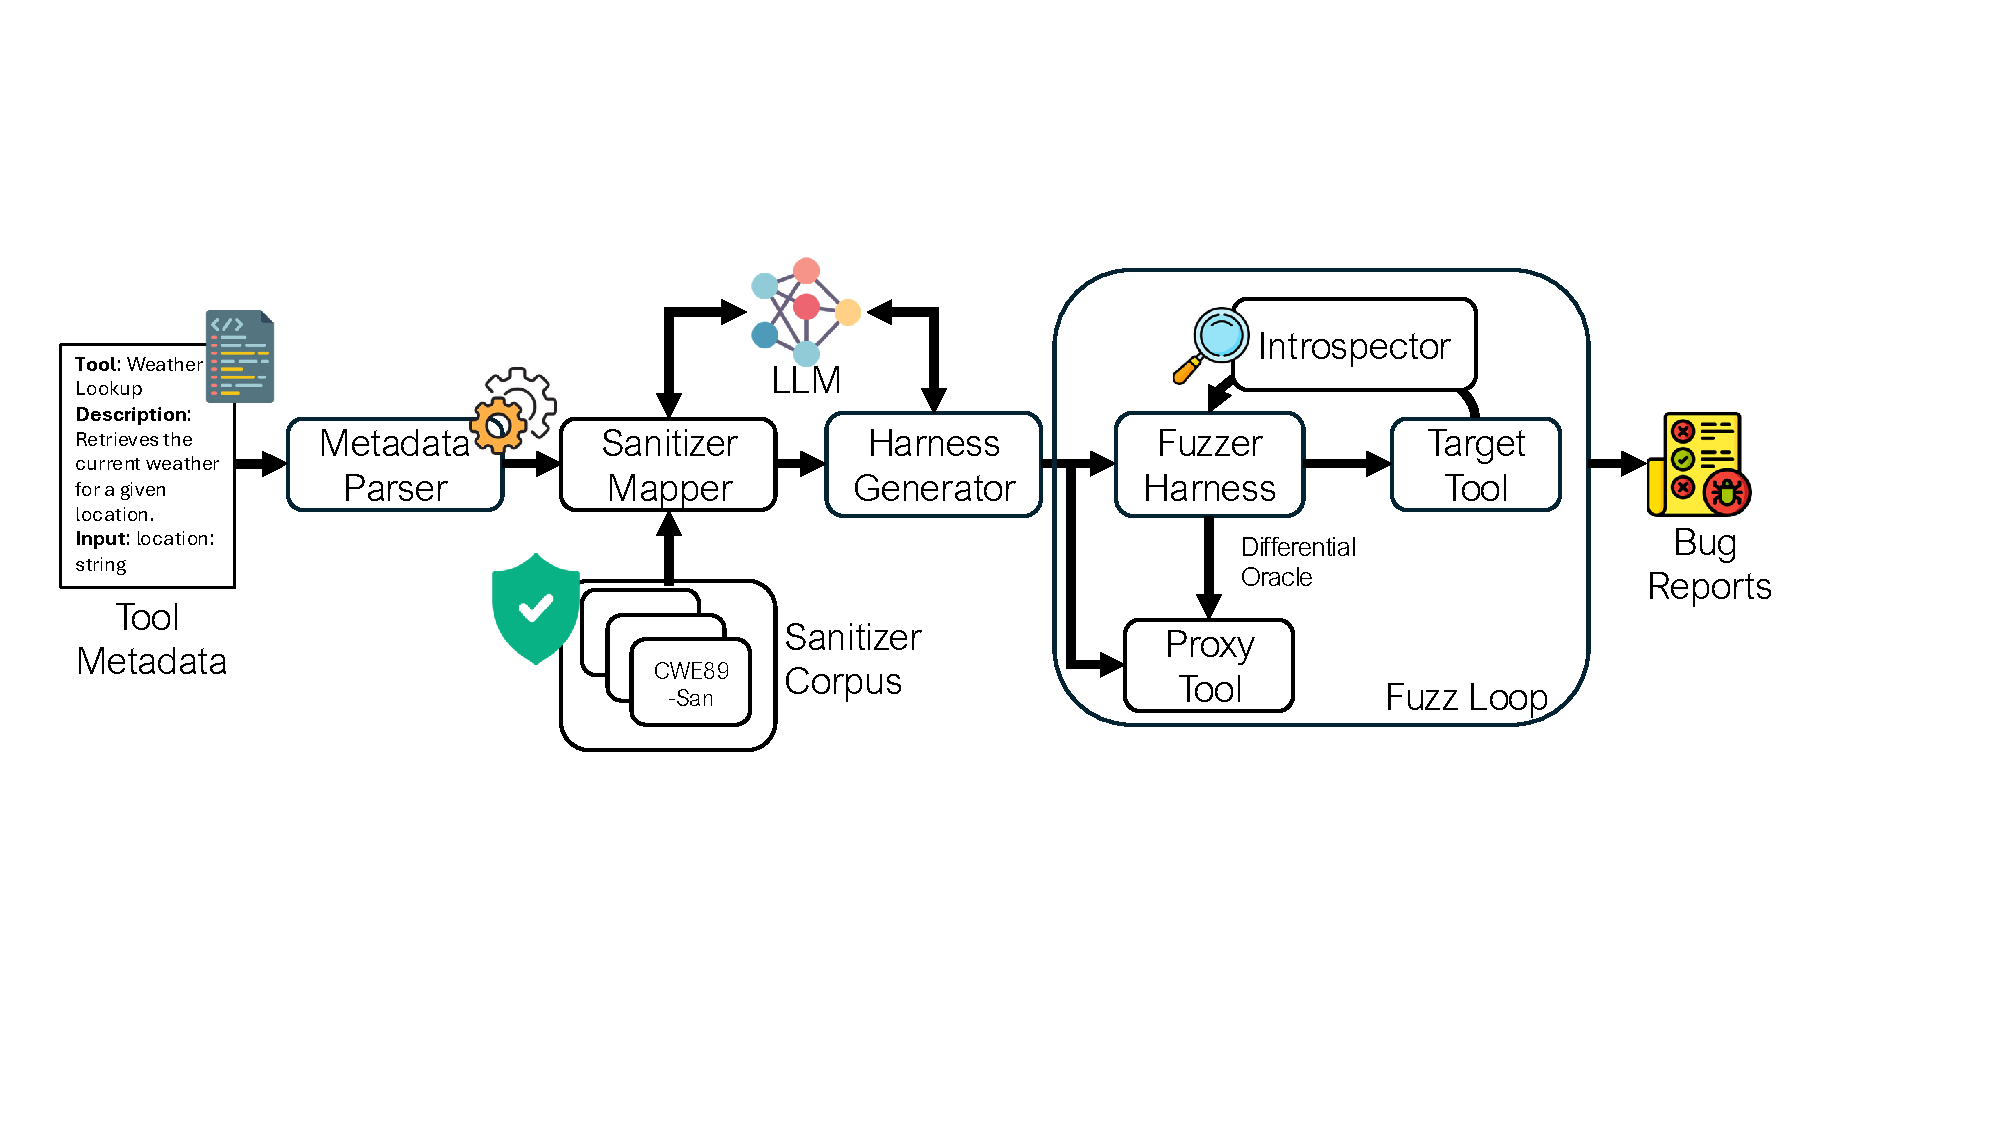
\includegraphics[width=\linewidth]{figs/overview.pdf}
\caption{\project{} maps tool metadata to semantics-aware sanitizers, generates
schema-valid fuzzing harnesses and, when needed, a proxy oracle, and detects
semantic security violations through runtime introspection or differential
checking.}
\Description{Pipeline diagram. A registered tool's metadata enters a Metadata Parser, which feeds a Sanitizer Mapper backed by a CWE-guided Sanitizer Corpus. The resulting specialized security specification drives a Harness Generator, which emits a schema-preserving Fuzzer Harness and, where needed, a Proxy Tool. A Fuzz Loop runs the harness against the target tool and reports violations via either a runtime Introspector or a Differential Oracle.}
\label{fig:tofu-overview}
\end{figure}

\project{} is a tool-aware fuzzing framework that turns the semantic
information already exposed by LLM tools into executable security tests.
As shown in Figure~\ref{fig:tofu-overview}, \project{} takes a registered
tool as input and automatically derives three artifacts: the security
properties to test, a harness that exercises those properties, and an oracle
that determines whether they are violated. \project{} operates through the
tool's existing orchestration interface, reusing its metadata discovery and
invocation mechanisms without requiring changes to the LLM or target tool.

The \textbf{Metadata Parser} first normalizes the tool description, argument
schemas, and natural-language argument descriptions. The \textbf{Sanitizer
Mapper} uses this information to associate each argument with applicable
checks from a CWE-guided \textbf{Sanitizer Corpus}. Each sanitizer couples a
semantic input class with adversarial inputs, an expected security property,
and the observations needed to establish a violation. For example, a path
argument can induce containment and traversal checks, while a URL can induce
scheme and destination checks. An LLM assists in mapping and specializing
these generic sanitizers to the semantics documented by the tool, but the
resulting sanitizer, rather than the LLM, defines the security oracle.

The specialized security specification drives the \textbf{Harness Generator}.
It constructs a \textbf{Fuzzer Harness} that mutates arguments while
preserving the target's schema, allowing adversarial values to traverse the
normal orchestration path and reach the implementation. For targets where
internal behavior cannot be observed, the generator additionally constructs a
\textbf{Proxy Tool} that encodes the expected behavior of the specialized
security checks. Thus, the same semantic specification determines both what
inputs are generated and what behavior is considered secure.

Finally, the \textbf{Fuzz Loop} executes generated invocations against the \textbf{Target Tool}. When implementation-level visibility is available, the \textbf{Introspector} observes sanitizer-relevant effects, such as filesystem, process, or network operations, and directly checks the corresponding property. Otherwise, the \textbf{Differential Oracle} compares the target against the generated proxy and identifies cases where the target accepts or processes an input that violates the inferred contract. Crashes and unhandled failures provide additional feedback. When a violation is detected, \project{} reports the triggering invocation, affected argument, expected property, and observed behavior. Section~\ref{sec:design} describes each stage in detail.

\section{Design}
\label{sec:design}

\project{} takes a registered tool and constructs a coverage-guided fuzzing target with automatically selected security checks from the information already exposed through
its orchestration interface. The design has four stages
(Figure~\ref{fig:tofu-overview}): (1) normalize the tool interface,
(2) select security sanitizers for each tool,
(3) generate schema-valid fuzzing inputs and the corresponding semantic
oracles, and (4) execute the target using conventional and semantic feedback.
Tool metadata informs both seed generation and sanitizer selection, ensuring that the property being exercised is also the property used to judge the execution.

\subsection{Metadata Extraction}
\label{sec:design-metadata}

\project{} begins from the metadata already exposed to the LLM. For a tool
$T$, the Metadata Parser constructs

\[
T = \langle D_T,\{a_1,\ldots,a_n\}\rangle,
\]

where $D_T$ is the tool-level description and each argument $a_i$ denotes an entry in the available input schema. The implementation retains the raw schema for use by the LLM and the input decoder, including argument names and types. The tool's natural-language description is additionally provided to the LLM for selecting sanitizers and generating seeds.

The parser obtains this information through the tool registry rather than
requiring a separate fuzzing specification. This is important because the
resulting representation captures exactly the interface presented to the LLM
and therefore the semantic contract that \project{} later tests.

% pierre
To handle the structural heterogeneity of tool interfaces across different ecosystems (e.g., MCP JSON-RPC declarations, LangChain and AutoGen Pydantic models, and FastMCP/Python type annotations), the Metadata Parser normalizes disparate definitions into a canonical, JSON-Schema-aligned representation. Primitive types (\texttt{string}, \texttt{integer}, \texttt{number}, \texttt{boolean}) and argument-level docstrings are extracted from schema fields or introspected signatures. For compound structures, such as nested objects and arrays, the parser recursively traverses sub-schemas (\texttt{properties} and \texttt{items}), preserving hierarchical access paths while exposing leaf-level attributes as distinct argument descriptors $a_i$ with their own natural-language contexts. Polymorphic parameters specified via unions (\texttt{oneOf}, \texttt{anyOf}, or Python \texttt{Union}) are preserved as multi-type disjunctions, allowing subsequent stages to specialize sanitizers and generate test cases for each candidate branch. Discrete value domains (\texttt{enum} and \texttt{Literal}) are retained as explicit finite sets to constrain baseline generation. Finally, the parser partitions arguments into required and optional sets based on schema constraints and the presence of default values $v_{\text{def}}$, enabling the harness generator to systematically alternate between partial invocations relying on defaults and fully specified adversarial payloads.

\subsection{Semantics-Aware Sanitizers}
\label{sec:design-mapper}

The central abstraction in \project{} is a \emph{semantics-aware sanitizer}.
Traditional sanitizers associate a program execution with a largely
application-independent property, such as whether a memory access is in
bounds. Tool vulnerabilities instead depend on what an input represents. A
string interpreted as a path requires different security checks from the same
string interpreted as a URL or command.

We represent a sanitizer as

\[
S = \langle A,G,O,I\rangle ,
\]

where $A$ is an \emph{applicability specification}, $G$ describes adversarial
input classes, $O$ defines the expected security property, and $I$ describes
the execution observations required to evaluate that property. The four
components deliberately connect input generation and bug detection. For
example, a filesystem-containment sanitizer may apply to path-like arguments,
generate absolute paths and traversal sequences, require that resolved
accesses remain beneath an allowed root, and request observations of
filesystem operations. A URL sanitizer instead generates adversarial schemes
and destinations and evaluates the resulting network behavior.

The initial Sanitizer Corpus organizes these specifications around recurring
CWE weakness classes. CWE is used as a source of reusable security knowledge,
not as the oracle itself: each corpus entry must translate a weakness into
concrete applicability conditions, input classes, expected behavior, and
observable evidence. Table \ref{tab:sanitizers} lists the CWE-based sanitizers used for \project{}. 

% pierre
\iffalse
\TODO{Pierre: describe the exact representation of a corpus entry. Include one
complete sanitizer example showing $A$, $G$, $O$, and $I$ as they appear in
the real system. Explain whether these fields are code, structured JSON,
natural language, or a combination.}
\fi
In \project{}, corpus entries are implemented as hybrid specifications combining declarative metadata for LLM interpretation with executable Python components for fuzzing and monitoring. Specifically, \textbf{Applicability ($A$)} is a structured JSON object with natural-language docstrings and semantic tags (e.g., associating CWE-22 with keywords like \texttt{path} or \texttt{directory}) consumed by the LLM during mapping. \textbf{Adversarial Generation ($G$)} provides structured JSON payload suites (e.g., \texttt{../../etc/passwd}, encoded escapes, and absolute paths) to guide mutation. \textbf{Security Oracle ($O$)} is an executable Python predicate (e.g., \texttt{check\_introspection\_path\_traversal}) evaluated against a behavioral rule (\texttt{on\_trigger: raise\_exception}), verifying that resolved filesystem accesses remain within an authorized root directory. \textbf{Execution Instrumentation ($I$)} comprises executable context-manager tracers (e.g., \texttt{FileAccessTracer} intercepting \texttt{builtins.open}) that collect concrete operations into the execution trace $\tau(T, x, I_S)$.

\subsection{Mapping Sanitizers}
\label{sec:design-specialization}

For each argument $a_i$, \project{} identifies the sanitizers whose
applicability conditions match its documented semantics:

\[
\mathcal{S}(a_i)=
\{S_j \mid S_j \text{ applies to } a_i\}.
\]

This decision cannot generally be made from the primitive type alone.
\project{} therefore considers the argument name, argument description,
schema, and surrounding tool description. An LLM interprets this
natural-language context and selects candidate sanitizers from the corpus.

The LLM does not decide whether an execution is vulnerable. Its role is
restricted to connecting an explicitly defined security property to an
argument whose semantics are expressed in natural language. The resulting
security decision remains grounded in the sanitizer's oracle.

To select the sanitizers used for a fuzzing campaign, the LLM is provided with the tool name, description, arguments, and the list of available sanitizers. The LLM then makes a selection based on which sanitizers are applicable to the likely classes of vulnerabilities for the tool.

% \TODO{Pierre - I don't believe there is any fallback or recourse for hallucinated or incorrectly added sanitizers currently. This can be impactful as well, as a file sanitizer on a tool meant to write outside of the work directory will be flagged. You should decide how you want to say this.}

If the LLM hallucinates by listing a non-existing sanitizer, \project{} detects it and simply does not add such sanitizer to the list. However, the LLM does not choose the expected sanitizers it will degrade the performance of \project{}, thus the choice of sanitizers made by the LLM has to be monitored to make sure results are accurate.

% \paragraph{Tool-specific specialization.}
% \TODO{Remove, no tool-specific specialization}
% Selecting a sanitizer identifies a general class of security property, but not
% necessarily its concrete policy. For example, filesystem containment requires
% a root directory, and a network-access check may require a set of permitted
% destinations. These values must be derived from the particular tool's
% interface.

% For every selected pair $(a_i,S_j)$, \project{} therefore produces a
% tool-specific sanitizer instance $S_{i,j}^{T}$. The instance retains the
% generic adversarial strategy and oracle structure of $S_j$, but binds
% tool-specific parameters inferred from $T$. A path argument described as
% ``within the current workspace,'' for example, specializes the generic
% containment property to the workspace associated with that tool.

% This specialization also allows \project{} to capture constraints more precise
% than the corresponding CWE. Tool metadata may restrict access to a particular
% directory, host, scheme, namespace, or service even though no standalone CWE
% encodes that exact policy.

% \TODO{Pierre: explain how specialization values are recovered in practice. For
% example, how does \project{} determine the concrete workspace root, allowed
% domain, or permitted resource set when the description uses relative or
% context-dependent terms? State what happens when the metadata does not contain
% enough information to instantiate the property.}

% \paragraph{Extending beyond the corpus.}
% \TODO{Remove, no sanitizer extension}
% A fixed sanitizer corpus would limit \project{} to weaknesses anticipated when
% the corpus was created. When metadata expresses a security restriction that
% does not match an existing sanitizer, \project{} may instead specialize a
% related sanitizer or construct a tool-specific condition from the documented
% constraint. Crucially, the generated condition must remain tied to an explicit
% property in the interface rather than to an unconstrained LLM judgment that an
% execution ``looks unsafe.''

% \TODO{Pierre: this is currently an important but underspecified claim. Explain
% exactly when \project{} is allowed to synthesize a new condition, the
% representation of the generated condition, how it becomes executable, and what
% prevents the LLM from inventing a security requirement not supported by the
% metadata. If the current implementation does not actually synthesize new
% sanitizers, remove this claim and present it as future work.}

\subsection{Schema-Aware Harness Generation}
\label{sec:design-harness}

Once \project{} has instantiated the applicable security properties, it
constructs a fuzzing harness for the tool. The harness operates on structured
arguments rather than on the serialized tool request. This distinction is
important: arbitrary byte-level mutations would frequently violate the
invocation schema and be rejected before reaching the implementation.

For each execution, the harness constructs a schema-valid invocation

\[
C = \langle T,\{a_1=v_1,\ldots,a_n=v_n\}\rangle
\]

and selects one or more arguments for semantic mutation. Values for the
selected arguments are generated using the corresponding sanitizer's
adversarial input classes, while the remaining arguments are populated with
values satisfying their declared schemas. A path sanitizer, for example, can
vary the path among traversal, absolute-path, normalization, and encoding
cases without corrupting the surrounding tool invocation.

This design separates \emph{structural validity} from \emph{semantic
adversariality}: the orchestrator should accept the invocation structurally,
allowing the test to exercise whether the tool itself enforces the stronger
security property.

The LLM is provided the target tool's description and arguments to construct a set of initial seeds following the tool's schema. With the initial corpus created, the fuzzer then follows a typical fuzzing campaign using Atheris and its built in mutation engine. The feedback mechanism uses coverage to capture interesting inputs, and captures crashing inputs either from sanitizer output or from actual crashes.

The seed generation is exclusively based on the LLM knowledge combined with the tool's basic information. The assumption is made that the tool is runnable in the current environment. 

\subsection{Semantic Oracles}
\label{sec:design-oracles}

A schema-valid malicious input is useful only if \project{} can determine
whether the resulting execution violates its intended property. Crashes,
exceptions, and conventional sanitizer failures remain useful signals, but
many target bugs terminate normally. \project{} therefore derives a semantic
oracle from the same specialized sanitizer used to generate the input.

\project{} evaluates the property through both runtime introspection and outcome sanitization.

\subsubsection{Runtime Introspection}
\label{sec:design-introspection}

When the target execution can be observed, the sanitizer specifies which
security-sensitive events are relevant to its oracle. For example,
filesystem-containment checks require the paths actually accessed by the
target, whereas SSRF checks require the destination actually contacted. The
Introspector collects only those event classes required by the active
sanitizer.

Let $\tau(T,x,I_S)$ denote the execution observations collected for target
$T$, input $x$, and sanitizer-required instrumentation $I_S$. The specialized
oracle evaluates

\[
O_S^T(\tau(T,x,I_S)) =
\begin{cases}
1 & \text{if the specialized property is violated},\\
0 & \text{otherwise}.
\end{cases}
\]

For containment, for example, the oracle can canonicalize an observed path and
test whether it escapes the specialized root. Thus, an execution that
successfully reads an unintended file becomes a fuzzing failure even though
the tool returns normally.

Each sanitizer has a mapping to introspection events from Python's introspection library to analyze the tool's behavior at runtime. The majority of these events are for Python runtime API hooking, enabling the fuzzer to observe file operations, system calls, and other interesting API usage based on the sanitizer.

Upon triggering an interesting event, the introspection hook adds details of the event to an internal list. The fuzzer then runs the corresponding sanitizers on the recorded events to check if an event is flagged as a violation. An input flagged by one of the sanitizers is then recorded and fuzzing continues.

Specifically, filesystem introspection hooks intercept raw file paths at the runtime API boundary (e.g., \texttt{open}) before path resolution occurs. The corresponding containment oracle then canonicalizes both the accessed path and the authorized base directory into their absolute, canonical forms (resolving relative traversals such as \texttt{../}, redundant separators, and symbolic links). By computing the relative path from the designated workspace root to the canonical target, the oracle accurately detects directory escapes and symlink traversals regardless of path encoding or aliasing tricks used by the fuzzed input.

\begin{table}[t]
\centering
\caption{Introspection hooks and monitored properties.}
\label{tab:introspection-hooks}
\small
\resizebox{\columnwidth}{!}{%
\begin{tabular}{ll}
\toprule
\textbf{Hook} & \textbf{Monitored Property} \\
\midrule
\texttt{FileAccess} & File access \& directory escape \\
\texttt{FileWrite} & Dangerous file creation \& upload \\
\texttt{TempFileLeak} & Uncleaned temporary files \\
\texttt{CommandExecution} & Command \& CLI flag injection \\
\texttt{CodeExecution} & Dynamic code evaluation \\
\texttt{Deserialization} & Unsafe object deserialization \\
\texttt{SQLExecution} & Raw / unparameterized SQL queries \\
\texttt{NetworkExecution} & Outbound requests \& SSRF \\
\texttt{SSLCertValidation} & Disabled TLS certificate checks \\
\texttt{UnrestrictedIPBinding} & Wildcard interface binding \\
\texttt{UnverifiedCodeDownload} & Code download without signature \\
\texttt{BlockingEventLoopCall} & Blocking calls in async loop \\
\texttt{ReDoS} & Catastrophic regex backtracking \\
\texttt{DataAmplification} & Decompression \& Zip bombs \\
\texttt{LoopCondition} & Unchecked loops \& CPU exhaustion \\
\texttt{NonceReuse} & Cryptographic Nonce/IV reuse \\
\texttt{WeakPRNG} & Insecure random generation \\
\texttt{WeakHash} & Broken hash algorithms (MD5/SHA1) \\
\texttt{SensitiveDataLogging} & Plaintext secrets in logs \\
\texttt{LogInjection} & CRLF / log forging sequences \\
\texttt{XXE} & XML entity expansion \\
\bottomrule
\end{tabular}%
}
\end{table}


\subsubsection{Outcome Sanitization}
\label{sec:design-differential}

In addition to introspection, \project{} uses selected sanitizers as \emph{contract-based outcome oracles}. A sanitizer evaluates the fuzzed input $x$ against a security policy and, when $x$ violates that policy, checks whether the target produced an appropriate safe outcome.

Let $V(x)$ denote that the sanitizer considers $x$ invalid or malicious, and let $\mathit{Reject}(T(x), E)$ denote that the target rejected $x$, where $E$ may include observed runtime side effects when available. The primary discrepancy of interest is

\[
V(x)
\quad\land\quad
\neg \mathit{Reject}(T(x), E).
\]

The oracle therefore answers a narrow question: according to the security contract derived from the tool interface, should this invocation have been accepted? The oracle may also treat network, process, or file-system side effects as evidence to whether an input was accepted or not. However, the most common check is a simpler input to output check for whether a target accepts a malicious input without raising an error or giving a safe fallback. 

Nondeterminism (e.g., dynamic timestamps or network latency) is mitigated by evaluating semantic invariants—such as structured error types and schema rejections—rather than brittle byte-level outputs. For tools with absent side effects (e.g., pure in-memory string or JSON transforms), the oracle relies on output validity predicates and execution health (catching unhandled exceptions or algorithmic stalls like ReDoS). For tools with ambiguous or silent outcomes, the oracle cross-references the tool's return status with runtime introspection traces (e.g., matching logged internal warnings or unperformed sink operations against reported success) to disambiguate whether the input was truly accepted.

\subsection{Fuzzing Loop and Feedback}
\label{sec:design-fuzzloop}

The fuzzing loop processes tools sequentially. For each tool, a list of appropriate sanitizers are chosen based on the tool's metadata, an initial seed corpus is generated, and the coverage-guided fuzzing engine is invoked. The engine continuously mutates inputs, which are mapped to the schema and executed by the fuzzer. Each execution is then evaluated for expanded coverage, a triggered crash, or sanitizer output.

An execution is interesting when it increases the measured coverage, guiding the input mutation toward deeper program states, while the oracle is responsible for determining if those states violate the security contract. Crash and sanitizer output classify an input as a potential failure or policy violation.

When \project{} detects a violation, the fuzzer records the triggering
invocation together with the sanitizer, expected property, and evidence that
caused the oracle to fire. These are outputs of the fuzzing process rather than
a separate architectural component.

% \subsection{Validating End-to-End Reachability}
% \label{sec:design-exploitation}
% \TODO{Remove, there isn't an actual end-to-end through the LLM running the tool to see if we can cause this in a real setup, the threat model is that the LLM can produce whatever}

% \project{} establishes that a tool implementation violates a security property
% for a concrete argument. Whether an attacker can cause that argument to reach
% the tool through an LLM agent is a separate question. Separating these two
% problems allows \project{} to test tools aggressively under the trust-boundary
% assumption established in Section~\ref{sec:trust-boundary}: every schema-valid
% tool argument may be attacker influenced, regardless of whether a particular
% prompt has already been identified that produces it.

% For discovered vulnerabilities, we separately test whether an attacker
% controlling natural-language input can induce the LLM to emit the triggering
% structured invocation through the normal orchestration path. This experiment
% establishes end-to-end exploitability but is not required for vulnerability
% discovery itself.

% \TODO{Pierre: describe the end-to-end validation procedure precisely:
% attacker capabilities, model inputs, whether the attacker supplies the tool
% name or schema, success criteria, number of trials/models, and any defenses or
% orchestration checks encountered. If the named Repeat-After-Me technique is
% retained, define it here only after giving this procedure.}


\section{Implementation}
\label{sec:implementation}
We implemented \textsc{ToFU} as an 8,400-SLOC Python framework (Table~\ref{tab:implementation-sloc}, excluding tests and libraries), running on Python 3.12, Atheris v2.3, LangChain Core v0.3, the official \texttt{mcp} SDK, and Node.js v20+.

\begin{table}[t]
\centering
\caption{Codebase breakdown by major component.}
\label{tab:implementation-sloc}
\small
\resizebox{\columnwidth}{!}{%
\begin{tabular}{llr}
\toprule
\textbf{Component} & \textbf{Modules \& Descriptions} & \textbf{SLOC} \\
\midrule
Sanitizers \& Oracles & \texttt{src/sanitizers/} (21 CWE introspection hooks \& checks) & 3,580 \\
Target Runners & \texttt{src/runners/} (In-process Python \& Node.js/MCP runners) & 2,700 \\
Fuzzing Engine & \texttt{src/fuzzer.py}, \texttt{src/input\_parser.py} (Schema-aware mutation) & 1,650 \\
Support \& Telemetry & \texttt{src/metrics.py}, \texttt{src/reporters.py}, \texttt{src/llm.py} (Seeding \& logs) & 470 \\
\midrule
\textbf{Total Core Code} & \textit{Excludes tests, prompts, and third-party tools} & \textbf{8,400} \\
\bottomrule
\end{tabular}%
}
\end{table}

\noindent\textbf{Sanitizer Specialization \& LLM Seeding.}
\textsc{ToFU} prompts \mbox{MiniMax M3} ($T=0.7$, up to 4 retries, fixed prompt in Appendix~\ref{sec:appendix-prompts}) with the target tool's metadata, JSON schema, and attack vectors from an internal seed bank to produce $N=6\text{--}12$ structured seeds. To synthesize valid binary documents, \textsc{ToFU} exposes native Python tool bindings (\texttt{reportlab} for PDF, \texttt{python-docx} for DOCX, \texttt{openpyxl} for XLSX, \texttt{zipfile} for archives); the LLM invokes these tools via standard function calling, materializing files to disk and referencing them as \texttt{predefined\_seed:<path>}. A deterministic fallback populates boundary numbers ($0, -1$), boolean toggles, and malformed types if the LLM fails ($<2\%$ of queries). Concurrently, \textsc{ToFU} matches schema properties against a 21-CWE corpus (\texttt{src/sanitizers/}), compiling executable Python verification predicates cached per schema hash.

\noindent\textbf{Fuzzing Engine \& Runtime Interception.}
\textsc{ToFU} recursively decodes libFuzzer-mutated byte streams into schema-valid arguments using \texttt{atheris.FuzzedDataProvider} (\texttt{FuzzInputParser}), mapping strings (\texttt{ConsumeUnicodeNoSurrogates}), numbers, arrays, objects, and deliberate type-mismatches. Feedback is measured as unique Python bytecode branch transitions via \texttt{sys.settrace} (and Atheris C-hooks), strictly filtering out framework internals (\texttt{src/fuzzer.py}, \texttt{src/sanitizers/}). To extract libFuzzer feature updates without disk I/O or terminal contention, C-level \texttt{stderr} is duplicated (\texttt{dup2}) into an IPC pipe drained asynchronously by a worker thread. Dual oracles evaluate each run: (1)~\emph{Runtime Introspection}, where \texttt{ExitStack} wraps execution sinks (\texttt{open}, \texttt{subprocess}, \texttt{socket}, \texttt{asyncio.get\_running\_loop}) to evaluate path containment, argument injection, and async loop freezing; and (2)~\emph{Black-Box Differential}, checking schema contracts and silent failures (\texttt{failed\_init\_non\_exit}).

\noindent\textbf{Target Execution \& Telemetry.}
\textsc{ToFU} supports in-process execution for Python tools (\texttt{PythonRunner}) and stdio subprocess workers for JS/TS MCP servers (\texttt{JSRunner}). Each iteration runs under a 5-second watchdog in an isolated temporary directory (\texttt{mkdtemp}) with environment variable restoration. Crashes are deduplicated by hashing the top-3 normalized target stack frames grouped by triggered sanitizer ID. Every trial logs execution latency, input values, triggered sanitizers, return status, edge coverage, and crash signatures.
\section{Evaluation}
\label{sec:eval}

\TODO{Pierre: Add explicit evaluation questions at the beginning. Right now the evaluation reports results without clearly connecting each subsection to the main claims made by ToFU. The questions should cover the applicability of the sanitizer corpus, semantic bug discovery, runtime filtering, fuzzing effectiveness, and real-world vulnerability discovery. You can phrase these based on the experiments that are already available.}

We structure our evaluation around the following research questions:

\noindent\textbf{RQ1 --- Sanitizer applicability.} To what extent can \project{}'s sanitizer corpus be mapped to the semantics exposed by real-world LLM tools?

\noindent\textbf{RQ2 --- Semantic bug detection.} Can \project{} detect violations of tool-specific semantic contracts that would not necessarily manifest as conventional crashes or schema violations?

\noindent\textbf{RQ3 --- Runtime filtering.} Can \project{} distinguish security-relevant semantic violations from benign runtime behavior observed during normal tool execution?

\noindent\textbf{RQ4 --- Fuzzing effectiveness.} Does coverage-guided mutation over schema-valid invocations reach the tool code paths that the selected sanitizers are meant to exercise, and does it surface semantic violations in real-world, publicly deployed tools?

We address RQ1 in Section~\ref{sec:eval-tools}, RQ2 and RQ3 in
Section~\ref{sec:eval-vulns}, and RQ4 in Section~\ref{sec:eval-coverage}.

\TODO{Pierre: Add an experimental setup subsection using the information already available. Report the machine configuration, operating system, Python and Node.js versions, number of cores used for each run, timeout policy, and fuzzing budget. Also state whether each reported result comes from a single run or multiple runs so that the methodology is explicit.}

% TODO(Nazmul): In a later evaluation revision, add repeated fuzzing trials for
% stochastic experiments and report an aggregate result and variance.

% TODO(Nazmul): In a later evaluation revision, add baseline and ablation
% experiments. At minimum compare full ToFU against ordinary Atheris or
% equivalent schema-guided fuzzing without semantic sanitizers and semantic
% runtime oracles. Separately evaluate the contribution of LLM seeding, the
% Seed Bank, sanitizer specialization, and semantic runtime checking.

\subsection{Tool selection}
\label{sec:eval-tools}
We evaluated our approach on 569 tools collected from 11 open-source
repositories. The repositories were chosen by taking the top MCP servers listed on https://github.com/mcp that could be fuzzed locally with simple setup. In addition, we've taken the first result when searching for "AI tool" on GitHub. 

\TODO{Pierre: The repository selection methodology needs to be reproducible. Define exactly what top MCP servers means, give the date on which this ranking was collected, report the initial candidate set if that information is available, and state the inclusion and exclusion criteria. In particular, define what could be fuzzed locally with simple setup means.}

\TODO{Pierre: The first result when searching for AI tool on GitHub is difficult to defend as a systematic sampling criterion. If this repository was included for a specific reason, explain that reason and treat it as an intentionally selected target rather than presenting the GitHub search result as part of a systematic sampling methodology.}

Table~\ref{tab:evaluation_repositories} details the complete breakdown of the 11 target repositories, spanning both native Python tools and Node.js MCP servers.

\begin{table}[h]
\centering
\caption{Breakdown of the 11 evaluated target repositories and tools.}
\label{tab:evaluation_repositories}
\begin{tabular}{lllr}
\hline
\textbf{Repository} & \textbf{Runtime} & \textbf{Description / Category} & \textbf{Tools} \\
\hline
\texttt{tools-main}          & Python     & Standalone Agent Tool Suite    & 412 \\
\texttt{pmb}                 & Python     & Memory \& Cognitive Graph MCP  &  68 \\
\texttt{serena}              & Python     & Workspace \& Coding Agent MCP  &  43 \\
\texttt{memo}                & Python     & Knowledge Graph \& Memory MCP  &  17 \\
\texttt{basic-memory}        & Python     & FastMCP Semantic Note Storage  &   9 \\
\texttt{markitdown}          & Python     & Document \& Media Converter    &   1 \\
\texttt{chroma-mcp}          & Python     & Vector Database Retrieval MCP  &   3 \\
\texttt{terravision}         & Python/JS  & Geospatial Visualization MCP   &   4 \\
\texttt{chrome-devtools-mcp} & Node.js/TS & Browser Automation MCP         &   6 \\
\texttt{DesktopCommanderMCP} & Node.js/TS & OS \& Terminal Control MCP     &   4 \\
\texttt{brightdata-mcp}      & Node.js/TS & Web Scraping \& Proxy MCP      &   2 \\
\end{tabular}
\end{table}

\TODO{Pierre: The dataset is heavily dominated by tools-main, which contributes 412 of the 569 tools. Acknowledge this explicitly and avoid using 569 tools as evidence of 569 independent projects or ecosystems. If the information is already available, also report the Python versus JavaScript and TypeScript breakdown and the major categories represented in the dataset.}

\TODO{Pierre: Add the exact repository revisions or commit hashes used in the evaluation. If some candidate tools from these repositories could not be evaluated, state how many were excluded and why. This is important for reproducibility.}

The tools used for evaluation were then all publicly-available tools, most of them being in projects with more than 1,000 GitHub stars.

\TODO{Pierre: Quantify most by giving the exact number of repositories or tools above this threshold. Also briefly explain why these repositories provide a useful sample of real LLM tools. GitHub stars can support evidence of visibility or adoption, but should not be used alone to claim representativeness.}

The analysis used 66 sanitizers in total: 45 CWE-based
sanitizers, 6 web-specific sanitizers, 5 MarkItDown-specific sanitizers,
5 HAR/ZIP-specific sanitizers, and 5 generic sanitizers.

\TODO{Pierre: This needs a careful methodology explanation because a reviewer may suspect target-specific overfitting. State when these 66 sanitizers were created and whether any sanitizer was added or modified after observing behavior or bugs in the evaluated targets. This is especially important for the MarkItDown-specific and HAR or ZIP-specific sanitizers because these formats also appear among the discovered vulnerabilities.}

\TODO{Pierre: Explain how the different sanitizer groups were obtained. In particular, distinguish sanitizers directly derived from CWEs, generic sanitizers, and format-specific sanitizers. The reader should understand whether the format-specific sanitizers are manually authored, generated from metadata, or specialized automatically by ToFU.}

% TODO(Nazmul): Later, evaluate sanitizer selection and specialization
% quantitatively. Across the evaluated tools, measure how many sanitizers ToFU
% considers applicable per tool or argument, how often specialization succeeds,
% and how often generated checks are irrelevant or invalid. Ideally manually
% label a representative sample and measure precision.

% TODO(Nazmul): Later, report how many of the 66 sanitizers are actually
% exercised during fuzzing and how many contribute to confirmed findings.

To seed the fuzzing process across these tools, TOFU employs two complementary input generators: (1) an LLM-guided generator equipped with 8 native binary document builders (\texttt{create\_pdf}, \texttt{create\_docx}, \texttt{create\_xlsx}, \texttt{create\_pptx}, \texttt{create\_zip}, \texttt{create\_xml}, \texttt{create\_html}, \texttt{create\_json}) and a categorized attack Seed Bank, and (2) a deterministic fallback mapper generating boundary numbers ($0, -1, 2^{31}-1, -2^{31}, \pm 10^{308}$), boolean permutations, empty structures, and type confusion payloads.

\TODO{Pierre: Add the corpus statistics that are already available. Useful information includes the number of initial seeds generated per tool, the number of tools requiring document builders, whether the LLM generator failed for any targets, and how often the deterministic fallback was used. If some of these statistics were not recorded, leave them for later rather than estimating them.}

% TODO(Nazmul): Later, add a seed-generation ablation comparing an empty or
% default corpus, deterministic fallback seeds, LLM-generated seeds, and the
% complete ToFU seed corpus. Measure coverage and semantic bug discovery.

\subsection{Found vulnerabilities}
\label{sec:eval-vulns}

Overall, the evaluation uncovered 14 vulnerabilities across five
repositories. These vulnerabilities span several distinct classes of
security-relevant behavior.

\TODO{Pierre: If these numbers are already available, report the funnel from ToFU observations to the final 14 findings. For example, state how many raw alerts were generated, how many unique candidates remained after deduplication, and how many were manually confirmed. This is useful for understanding the amount of manual triage. Do not add numbers that were not recorded.}

\TODO{Pierre: Add the current disclosure and validation status for each finding. Indicate whether each issue has been reported, acknowledged, fixed, or assigned a public issue, advisory, or CVE where applicable. Maintainer confirmation will strengthen the vulnerability claims.}

First, three vulnerabilities involve unintended access to local resources
through interfaces that are expected to manipulate remote resources. In
particular, tools accepting URLs may also accept \texttt{file://} URIs,
allowing local files to be opened or rendered.

A second category consists of unsafe filesystem operations. Two
vulnerabilities allow attacker-controlled input to influence where files
are written: one through an insufficiently constrained output path and
another through path traversal during HAR/ZIP extraction.

Four vulnerabilities affect availability and robustness. Malformed or
unexpected inputs can terminate the tool or MCP server through
\texttt{sys.exit}, uncaught exceptions, invalid filesystem strings, or
failed assertions. Because MCP servers may expose several tools through a
single long-running process, such failures can affect more than the
individual tool invocation that triggered them.

Two additional vulnerabilities concern trust-boundary and initialization
failures: one component communicates with another process without requiring
authentication, while another fails open when initialization of its
language-server dependency fails.

The remaining three vulnerabilities concern resource and interface
hygiene: a temporary file is not removed after use, attacker-controlled
strings are written to logs without escaping, and one tool relies on a
deprecated MCP SDK annotation.

\TODO{Pierre: Establish the security impact of each category under the paper's threat model. State who controls the triggering input, what privilege the tool or MCP server has, and what security property is violated. This is especially important for the temporary-file cleanup issue, log injection, and deprecated API finding because reviewers may otherwise classify these as reliability or software-quality issues rather than security vulnerabilities.}

We classify the 14 identified issues into two categories: 
\begin{itemize}
    \item Semantic Input Validation Vulnerabilities (9 issues), which require specialized argument-level semantic payloads and runtime introspection oracles to be discovered
    \item Architectural and Lifecycle Defects (5 issues), which manifest as process-level design flaws, improper error recovery, or missing IPC authentication independent of specific tool argument payloads
\end{itemize} 

\TODO{Pierre: Explain exactly how the five Architectural and Lifecycle Defects were discovered. Because the text says that these defects are independent of specific tool argument payloads, the reader needs to know whether they were automatically detected by initialization or runtime telemetry, surfaced while investigating another ToFU alert, or found through manual analysis. Be precise about what ToFU itself discovered.}

% TODO(Nazmul): Later, evaluate the nine Semantic Input Validation
% Vulnerabilities under baseline and ablated fuzzing configurations. Use a
% fixed fuzzing budget and report whether each configuration finds each bug
% and the corresponding time to discovery.

To isolate these 14 genuine flaws from benign runtime activity, TOFU pairs each sanitizer with an explicit behavioral rule (\texttt{raise\_exception}, \texttt{allow\_success\_with\_fallback}, or \texttt{allow\_success\_always}) and workspace boundary constraints. This semantic filtering suppresses normal telemetry noise (e.g., reading configuration files like \texttt{.env} or executing \texttt{git rev-parse HEAD} during framework startup) while flagging contract violations.

\TODO{Pierre: Explain how these behavioral rules are assigned to sanitizers and give enough information to understand why the examples listed here are considered benign. If the counts are already available, report how much filtering occurs before the final alerts are produced.}

% TODO(Nazmul): Later, quantitatively evaluate semantic filtering. Compare the
% number of raw intercepted events or candidate violations before filtering
% against the number remaining afterward and the number of confirmed findings.

% TODO(Nazmul): Later, add an oracle ablation against a naive policy that
% flags every intercepted sensitive operation. Measure alert volume and false
% positives to show the value of ToFU's semantic behavioral rules.

The 14 found vulnerabilities are listed in table \ref{tab:identified_issues}. The most critical ones allow to crash the MCP server, to access the MCP server local files, to overwrite its existing files or to saturate its storage space, and to store files outside of intended directory when decompressing a compressed archive.

\begin{table}[h]
\centering
\caption{Summary of identified issues.}
\label{tab:identified_issues}
\begin{tabular}{llll}
\hline
\textbf{Project} & \textbf{Component} & \textbf{Class} & \textbf{Semantic} \\
\hline
tools & \texttt{http\_check} & Local file access & Yes \\
markitdown & \texttt{convert\_to\_markdown} & Local file access & No \\
tools & \texttt{extract\_issues} & Unhandled process termination & Yes \\
chrome-devtools-mcp & \texttt{navigate\_page} & Local resource access & No \\
tools & \texttt{extract\_issue\_numbers} & Uncontrolled output path & Yes \\
tools & \texttt{extract\_issue\_numbers} & Improper input validation & Yes \\
tools & \texttt{extract\_har} & Path traversal & Yes \\
tools & \texttt{extract\_har} & Unhandled malformed archive & Yes \\
serena & Task executor & Resource cleanup issue & No \\
serena & Task executor & Log injection & No \\
serena & \texttt{FindSymbolTool} & Invalid input handling & Yes \\
serena & JetBrains client & Missing authentication & No \\
serena & Project query tools & Fail-open initialization & No \\
memo & \texttt{memo\_version} & API compatibility issue & No \\
\hline
\end{tabular}
\end{table}

\TODO{Pierre: Expand this table if the relevant information is already available, or add a second table, to better connect each finding to how ToFU detects it. Useful fields include the violated property or CWE, triggering condition, sanitizer or oracle responsible for detection, whether a fuzzing input is required, and disclosure status. The important connection is from ToFU mechanism to triggering input or condition to observed behavior to confirmed vulnerability.}

\TODO{Pierre: Explicitly state that the 14 entries correspond to distinct root causes and briefly explain the deduplication methodology. Several findings occur in the same component, so the reader needs to understand why they are counted as separate vulnerabilities.}

\TODO{Pierre: Add a short quantitative summary using information that is already available, such as the number of affected repositories, affected tools, semantic findings, input-independent findings, and findings acknowledged or fixed by maintainers.}

% TODO(Nazmul): Later, add time-to-discovery and baseline-discovery results to
% the vulnerability table once repeated comparative runs are available.

\subsection{Code coverage}
\label{sec:eval-coverage}
Figure~\ref{fig:coverage-tools} shows the proportion of code covered after 24-hour runs for several tools. Depending on the amount of total features in the tool, the coverage has either reached its final coverage almost instantly, or has taken hours to reach its final number. In both cases, most of the coverage for the tool features was reached in less than an hour. Code coverage is strictly scoped to the first-party source code of each target tool/repository, explicitly excluding third-party dependencies, standard runtime libraries, and test suites.

\TODO{Pierre: Explain why these particular tools were selected for the coverage figure. State whether they were chosen as representative examples, because coverage instrumentation was available, or according to another criterion. This is important because the evaluation contains 569 tools but the figure reports only a small subset.}

\TODO{Pierre: Define the coverage metric and denominator precisely. The current discussion refers to features, branch coverage, and basic blocks. These terms should not be used interchangeably. Explain exactly what is measured, how the total first-party code is calculated, and what the basic-block number shown in each bar represents.}

\TODO{Pierre: The text states that most coverage was reached in less than one hour, but the current figure reports only the final 24-hour result. If you already have the time-series data described in the Implementation section, either show it or avoid making a stronger temporal claim than the presented figure supports.}

\TODO{Pierre: Be careful when describing Python and JavaScript coverage. If the two runners use different coverage definitions, explain the difference and avoid presenting their percentages as directly comparable.}

% TODO(Nazmul): Later, replace or complement the final coverage bars with
% coverage-over-time comparisons against the baseline and relevant ablations.

% TODO(Nazmul): Later, consider a semantic coverage metric, such as the number
% of applicable sanitizers exercised, sensitive operations reached, or
% semantic oracle conditions exercised. Structural code coverage is only an
% indirect measure of ToFU's central contribution.


Across these targets, TOFU operates with two execution runners:
\begin{itemize}
    \item \textbf{In-Process Python Runner (\texttt{PythonRunner}):} Dynamically invokes Python functions directly within the fuzzer process, enabling over 20 low-overhead introspection context-manager tracers (intercepting \texttt{open}, \texttt{subprocess.Popen}, \texttt{eval}, etc.).
    \item \textbf{Socket-Driven Node.js Runner (\texttt{JSRunner}):} Executes JavaScript/TypeScript MCP servers as child processes communicating over Unix domain sockets (\texttt{coverage\_wrapper.js}). It collects V8 branch coverage at runtime and forwards it to the Atheris engine via an in-memory trampoline (\texttt{fake\_coverage.py}).
\end{itemize}

\TODO{Pierre: Most of the runner mechanism belongs in the Implementation section. In this section, retain only the details necessary to explain how coverage is collected for the two runtime environments.}

% TODO(Nazmul): Later, measure fuzzing throughput for representative Python and
% JavaScript targets and quantify the overhead of semantic runtime
% introspection by comparing executions per second with tracers enabled and
% disabled.

% TODO(Nazmul): Later, validate the JavaScript coverage-feedback mechanism by
% comparing representative JavaScript targets with V8-to-Atheris feedback
% enabled and disabled. This will show whether the forwarded coverage improves
% exploration rather than merely recording executed branches.

\begin{figure}[htbp]
\centering

\resizebox{0.98\columnwidth}{!}{%
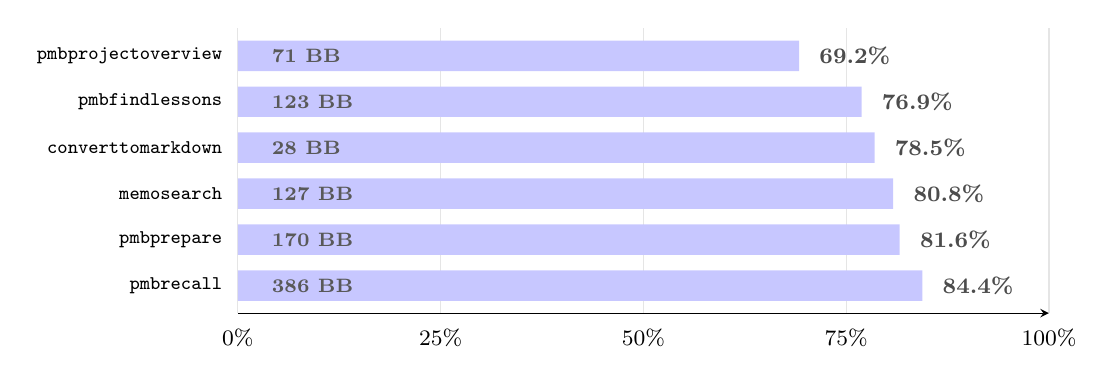
\begin{tikzpicture}

\begin{axis}[
    xbar,
    width=0.98\columnwidth,
    height=5.2cm,
    xmin=0,
    xmax=100,
    ymin=-0.6,
    ymax=5.6,
    y dir=reverse,
    xtick={0,25,50,75,100},
    xticklabels={0\%,25\%,50\%,75\%,100\%},
    ytick={0,1,2,3,4,5},
    yticklabels={
        \texttt{pmbprojectoverview},
        \texttt{pmbfindlessons},
        \texttt{converttomarkdown},
        \texttt{memosearch},
        \texttt{pmbprepare},
        \texttt{pmbrecall}
    },
    bar width=11pt,
    axis x line=bottom,
    axis y line=left,
    y axis line style={draw=none},
    xmajorgrids=true,
    grid style={gray!20},
    tick style={draw=none},
    tick label style={font=\footnotesize},
    yticklabel style={font=\scriptsize},
    clip=true
]

% Bars
\addplot[
    fill=blue!22,
    draw=none
] coordinates {
    (69.2,0)
    (76.9,1)
    (78.5,2)
    (80.8,3)
    (81.6,4)
    (84.4,5)
};

% Number of basic blocks
\node[
    anchor=west,
    font=\scriptsize\bfseries,
    text=black!65
] at (axis cs:3,0) {71 BB};

\node[
    anchor=west,
    font=\scriptsize\bfseries,
    text=black!65
] at (axis cs:3,1) {123 BB};

\node[
    anchor=west,
    font=\scriptsize\bfseries,
    text=black!65
] at (axis cs:3,2) {28 BB};

\node[
    anchor=west,
    font=\scriptsize\bfseries,
    text=black!65
] at (axis cs:3,3) {127 BB};

\node[
    anchor=west,
    font=\scriptsize\bfseries,
    text=black!65
] at (axis cs:3,4) {170 BB};

\node[
    anchor=west,
    font=\scriptsize\bfseries,
    text=black!65
] at (axis cs:3,5) {386 BB};

% Percentages
\node[
    anchor=west,
    font=\footnotesize\bfseries,
    text=black!70
] at (axis cs:70.5,0) {69.2\%};

\node[
    anchor=west,
    font=\footnotesize\bfseries,
    text=black!70
] at (axis cs:78.2,1) {76.9\%};

\node[
    anchor=west,
    font=\footnotesize\bfseries,
    text=black!70
] at (axis cs:79.8,2) {78.5\%};

\node[
    anchor=west,
    font=\footnotesize\bfseries,
    text=black!70
] at (axis cs:82.1,3) {80.8\%};

\node[
    anchor=west,
    font=\footnotesize\bfseries,
    text=black!70
] at (axis cs:82.9,4) {81.6\%};

\node[
    anchor=west,
    font=\footnotesize\bfseries,
    text=black!70
] at (axis cs:85.7,5) {84.4\%};

\end{axis}
\end{tikzpicture}%
}

\caption{Code coverage after 24 hours.}
\Description{Horizontal bar chart of branch coverage reached after 24 hours of fuzzing on each evaluated target, with per-bar percentage labels.}
\label{fig:coverage-tools}
\end{figure}

% TODO(Nazmul): Later, add a bug-discovery effectiveness experiment for the
% semantic vulnerabilities. Under a fixed budget and repeated trials, report
% discovery success and time to discovery for full ToFU and the baseline.
% This is more directly tied to the security contribution than final code
% coverage alone.

% TODO(Nazmul): Later, add a compact ablation summary isolating the
% contributions of sanitizer specialization, LLM and Seed Bank input
% generation, semantic runtime oracles, and coverage-guided mutation.


\section{Case Study}
\label{sec:casestudy}

\TODO{Pierre: The current section explains the vulnerability well, but it does not yet function as a case study of ToFU. The key purpose of this section should be to walk through the complete discovery process. Explain what metadata ToFU receives for this tool, which sanitizer is selected and why, what input or seed is generated, how fuzzing transforms that input into the triggering argument, what runtime operation the introspection layer observes, and why the semantic oracle identifies that operation as a violation. The reader should be able to follow the bug from tool metadata all the way to the final vulnerability.}

\TODO{Pierre: At the beginning of the case study, briefly explain why this particular bug is representative of ToFU's contribution. The interesting point is not simply that command-line argument injection exists, but that the argument is syntactically a valid string and is passed safely without a shell, while its semantic interpretation by the downstream command violates the intended tool contract. This is exactly the distinction the paper should emphasize.}

An example of a vulnerability found using \project{} that can be studied can be found in \texttt{tools-main/\allowbreak python/\allowbreak extract\_issues.py}. 

\TODO{Pierre: Before the code listing, describe the tool's documented interface. State what range\_spec is supposed to represent according to the tool metadata or description and, if available, include the relevant description supplied to ToFU. This establishes the intended semantic contract before showing how the implementation violates it.}

\begin{lstlisting}[
  basicstyle=\ttfamily\small,
  breaklines=true,
  columns=fullflexible,
  linewidth=\linewidth
]
def extract_issue_numbers(range_spec: str) -> str:
    ...
    git_range = range_spec if ".." in range_spec else f"{range_spec}..HEAD"
    ...
    result = subprocess.run(
        ["git", "log", git_range, "--pretty=%B"],
        capture_output=True,
        text=True,
        check=True,
    )
    ...

\end{lstlisting}

\TODO{Pierre: Immediately after the listing, connect this code to ToFU rather than moving directly to manual vulnerability analysis. Explain which sanitizer ToFU associates with range\_spec and why the tool metadata makes that sanitizer applicable. If ToFU specializes a generic CWE-88 sanitizer to this argument, show the resulting check or summarize it here. This is the most important missing step in the current case study.}

In this case, range\_spec is expected to be a string representing either a single tag/commit or an explicit Git range.

\TODO{Pierre: Explain how this expectation is known. Ideally tie it directly to the tool description, argument metadata, documentation, or generated sanitizer. This is important because ToFU's claim is that the security property follows from documented tool semantics rather than a manually written specification.}

By default, \texttt{subprocess.run} is invoked with a list of arguments and without a shell interpreter (\texttt{shell=False}); therefore, classic command chaining and shell injection (e.g., providing \texttt{range\_spec="; echo success"} or piping operators) are inherently prevented.

\TODO{Pierre: This distinction is important and should be connected explicitly to the motivation for semantic sanitization. A conventional command-injection check looking for shell metacharacters would consider this invocation substantially safer because shell interpretation is disabled. ToFU instead needs to reason about the semantics of the argument accepted by Git itself. Make that point explicit.}

However, passing unsanitized arguments directly into a command invocation opens the door to \textit{CLI Argument Injection} (CWE-88). Because the argument is passed as a standalone vector element to \texttt{git}, an input formatted as a command-line flag (such as \texttt{--output=/user/../user/foo}) causes the \texttt{git} binary to interpret the parameter as an operational option rather than a positional revision range. Under this flag, \texttt{git log} redirects its formatted output directly to the specified file path on disk.

\TODO{Pierre: Show the actual triggering input produced by ToFU, preferably exactly as recorded by the fuzzer after minimization. If the example shown here is the actual minimized input, state that explicitly. If it is only an illustrative input, replace it with or separately show the real input. A case study should distinguish the discovered proof of concept from an explanatory example.}

\TODO{Pierre: Explain how ToFU's runtime oracle detects this behavior. For example, if the introspection layer observes the file creation or the subprocess arguments, state exactly what event is intercepted and what rule causes ToFU to flag it. The current text explains why the behavior is vulnerable, but not how ToFU automatically recognizes the violation.}

\TODO{Pierre: Also explain whether ToFU recognizes the dangerous command-line option before execution or detects its effect afterward through runtime introspection. This distinction matters for understanding the architecture and should match the Design section.}

Furthermore, the ternary check on line 3 (\texttt{range\_spec if ".." in range\_spec else f"\{range\_spec\}..HEAD"}) is subverted by directory traversal sequences: providing path traversal dots (\texttt{..}) in the file path satisfies the substring condition, thereby bypassing the automatic appending of \texttt{..HEAD} and passing the adversarial \texttt{--output} argument verbatim to the subprocess on line 6.

\TODO{Pierre: There appears to be a LaTeX or code-formatting issue in the inline expression in this sentence. Check the nested texttt commands and braces carefully. I am not changing it here because the existing text should remain untouched, but this line should be fixed before submission.}

\TODO{Pierre: Clarify that the two dots are useful here because the implementation checks only whether the string contains two consecutive dots. The security problem is not conventional path traversal by itself. The dots also manipulate the program's branch condition so that the injected Git option is passed unchanged. That interaction is an interesting semantic aspect of the bug and is worth emphasizing.}

\TODO{Pierre: If ToFU generated or mutated the two-dot sequence automatically, explain that transition here. Showing how the fuzzer reaches the final option while satisfying the program's range check would make this a much stronger fuzzing case study.}

Although this vulnerability does not provide direct arbitrary code execution, it presents serious security and operational risks that can be exploited by an attacker in two distinct ways:

\noindent
\textbf{Denial of Service through Storage and Inode Exhaustion (CWE-400):} By repeatedly invoking the tool with distinct file names or deeply nested paths across the filesystem, an attacker can generate a large volume of output files. This continuous file generation can quickly saturate available disk space or exhaust filesystem inodes, ultimately causing denial of service for the MCP server and co-located services.

\noindent
\textbf{Arbitrary File Overwrite and Asset Integrity Corruption (CWE-732):} Depending on the filesystem permissions granted to the MCP server process, an attacker can overwrite existing critical files, such as configuration files, local database snapshots, or application assets. The overwritten files will contain the formatted \texttt{git log} commit history (\texttt{--pretty=\%B}) rather than their original contents. Consequently, any subsequent process or service attempting to read or parse these corrupted files will encounter unexpected structures and fail, inducing silent runtime errors, degraded application behavior, or complete subsystem crashes.


\TODO{Pierre: Recheck the CWE classification for the arbitrary-file-overwrite consequence. CWE-732 is Incorrect Permission Assignment for Critical Resource, which does not appear to describe the root cause here because the vulnerability does not assign incorrect file permissions. CWE-88 already captures the argument-injection root cause. If you want a secondary CWE for the resulting filesystem behavior, select one that actually corresponds to uncontrolled file path or file modification rather than permission assignment.}

\TODO{Pierre: Be careful with the claim about deeply nested paths. State only behavior that was actually validated. Git can write to a supplied output path, but this does not necessarily imply that it creates arbitrary missing parent directories. The denial-of-service argument does not need this stronger claim because repeatedly creating distinct files in writable existing directories is sufficient to explain storage or inode exhaustion.}

\TODO{Pierre: Close the case study with a short paragraph explaining why this bug illustrates ToFU's broader value. The key observation is that the parameter is type-correct, the subprocess invocation avoids shell interpretation, and ordinary malformed-input checking may therefore see nothing unusual. The vulnerability appears only when the string is interpreted according to Git's command-line semantics and compared against the intended meaning of range\_spec. Connect this explicitly back to the LLM-to-tool trust boundary and semantic sanitizer design.}

% TODO(Nazmul): Later, replay this vulnerability under a conventional Atheris
% or schema-guided fuzzing configuration without ToFU's semantic seeding and
% sanitizer guidance. Report whether the baseline discovers the argument
% injection under the same budget and compare time to discovery.

% TODO(Nazmul): Later, separately disable the semantic runtime oracle for this
% case study and determine whether the triggering input would otherwise appear
% as an ordinary successful tool execution. This would provide a particularly
% clear demonstration of why semantic runtime checking is necessary.

% TODO(Nazmul): If the original fuzzing logs retain the mutation history or
% corpus evolution, reconstruct the progression from the initial seed to the
% minimized --output triggering input. This could provide a useful concrete
% example of how ToFU's seeding and coverage-guided mutation cooperate.


\section{Discussion}
\label{sec:discussion}
\noindent\textbf{Multi-Agent Systems.}
\project{} currently targets tool invocations made through an LLM orchestration framework. However, emerging multi-agent systems may distribute tool use across multiple interacting agents. For example, one agent may invoke a tool and pass its result to another agent, which subsequently uses the result as an argument to a different tool. Supporting such systems requires extending \project{} from individual tool invocations to multi-agent execution paths. One possible approach is to construct a harness over the agent communication graph and fuzz both agent-to-agent messages and the tool invocations reachable from each agent. The tool-specific sanitizers generated by \project{} can remain unchanged, but must be applied at each tool boundary reached during the execution. Furthermore, testing multi-agent executions requires maintaining state across multiple agent and tool invocations. We leave support for multi-agent systems to future work.

\noindent\textbf{Coverage of Third-Party Components.}
Many tools are lightweight wrappers around external libraries, services, or applications. For example, a browser tool may contain only a small amount of orchestration code while most of its functionality executes inside Chromium. In such cases, coverage collected only from the tool implementation does not capture how extensively the underlying component is exercised. \project{} can be extended with component-specific coverage collectors that combine coverage from the tool implementation and its dependencies. For example, browser tools could additionally collect Chromium coverage, while tools invoking native libraries could collect coverage from instrumented library code. \project{} can then use the combined coverage when deciding whether a generated input exposes new behavior. Supporting arbitrary third-party components requires component-specific instrumentation interfaces, which we leave for future work.

\noindent\textbf{Stateful Tool Interactions.}
\project{} currently fuzzes tools by generating inputs for individual tool interfaces. However, some tool behavior depends on state established by previous invocations. For example, one tool invocation may create a resource that is subsequently modified, queried, or deleted by another invocation. Bugs involving such state may therefore require a sequence of otherwise valid tool calls. \project{} can be extended to generate multi-call harnesses by identifying relationships between tool arguments and outputs, such as a resource identifier returned by one tool and consumed by another. The fuzzer can then mutate both the arguments and ordering of calls while applying the existing semantic sanitizers at each tool boundary. Determining useful invocation sequences across large tool collections remains an open problem, and we leave stateful tool fuzzing to future work.

\section{Related Work}

\paragraph{Attacks that deliver adversarial values to a tool.}
One line of work asks how an adversarial value reaches a tool in the first place, treating the tool itself as a black box that faithfully executes whatever it receives. Adversarial suffixes~\cite{zou2023universal} and indirect prompt injection through retrieved content~\cite{greshake2023not} manipulate what the model decides to send; ToolHijacker~\cite{toolhijacker} and MPMA~\cite{wang2026mpma} instead manipulate \emph{which tool} gets selected, by impersonating or out-competing a legitimate tool's description, and WebInject~\cite{wang2025webinject} shows the same idea survives a change of modality by perturbing screenshot pixels rather than text. Les Dissonances~\cite{les-dissonances} pushes delivery downstream further still, letting one tool's output contaminate a sibling tool's arguments within a session. AgentDojo~\cite{debenedetti2024agentdojo} consolidates these attacks and a growing set of defenses into a shared dynamic benchmark. All of this work asks whether an agent's \emph{decision} can be steered; TOFU instead assumes an adversarial value has already arrived at the tool boundary through any such channel (or through mere carelessness, our A1) and asks whether the \emph{implementation} enforces the security property its interface claims -- a defense that stopped every attack above would still leave TOFU's semantic bugs exploitable by a careless caller, and a tool hardened against every bug TOFU finds is still exposed if its description can be spoofed at selection time.

\paragraph{Defenses, and cataloging the {MCP} threat landscape.}
A second line of work defends against exactly these delivery attacks rather than examining what a tool does once invoked: pre-filtering and localizing injected content~\cite{shi2025promptarmor,jia2026promptlocate}, training models to respect a privilege hierarchy over instruction sources~\cite{wallace2024instruction}, and reconstructing least-privilege permission scopes at the orchestration layer~\cite{zhu2025miniscope}. None of this checks that a tool, once invoked through a permitted channel, behaves according to its own documented semantics; Model-Carrying Code~\cite{sekar2003model} is an early, non-LLM precursor to that idea; TOFU's differential oracle plays a similar role but derives the contract automatically from natural-language tool metadata. A parallel body of survey, taxonomy, and infrastructure work catalogs the broader landscape without testing any single deployment directly~\cite{hou2025landscape,li2026towards,trustshiftprobe,aclemcp,web3survey}: MCPXKIT~\cite{guo2026systematic} unifies 31 attack methods into a single framework (IEEE TDSC); Song et al.~\cite{song2025beyond} give the first end-to-end empirical study of the MCP supply chain, from malicious-server upload through popular aggregator platforms to local exploitation; and MCPCorpus~\cite{lin2025mcpcorpus} contributes the data layer underneath all of this, a publicly released snapshot of roughly 14,000 MCP servers with normalized registry and repository metadata. Within that body, Ding et al.~\cite{aclemcp} argue that remote tool use needs attested, expiring capability leases rather than ambient trust, Rostamzadeh et al.~\cite{trustshiftprobe} characterize \emph{staged} trust attacks in which a server behaves benignly until trust is established, and AEGIS~\cite{aegis} targets cross-domain resource abuse specifically. These establish \emph{that} contracts can be violated in many ways; TOFU complements them with a mechanism for deriving and testing a specific tool's contract automatically.

\paragraph{Catalog-bounded scanners and large-scale dynamic measurement.}
The systems closest to TOFU's stated goal each start from a fixed, predetermined list of weaknesses or sinks: static analyses that never execute the target~\cite{mcp-first-glance,mcp-seclint}, a broad regex rule corpus~\cite{agentthreatrules}, and MCP-Scanner~\cite{mcp-scanner}, which does execute tools but only against a catalog of known threats (Cisco AI Defense's unaffiliated, identically-named open-source tool -- which we refer to as Cisco MCP Scanner~\cite{cisco2025mcpscanner} to avoid confusion with the academic tool above -- follows the same catalog-bounded pattern at industrial scale, layering YARA rules, LLM-based description review, and a cloud threat-intelligence API). MCPSecBench~\cite{yang2025mcpsecbench} systematizes this same catalog-driven approach into a benchmark, useful for comparing scanners but bounded, like them, by its enumerated categories. As Table~\ref{tab:motivation} summarizes, none derives its checks from a tool's own argument semantics. The most closely related contemporaneous work instead moves to dynamic, large-scale measurement, and is where TOFU's contribution most needs careful delineation: VIPER-MCP~\cite{viper-mcp} pairs CodeQL taint queries with an LLM-driven agent that evolves natural-language prompts until an attacker-controlled value provably reaches a sink at runtime, reporting 106 zero-days and 67 assigned CVEs across roughly 39{,}884 repositories -- a scale no single-institution study matches. It is the closest system to \project{}, and the distinction is not scale but what a check can express: VIPER-MCP models exactly three taint-style classes (command injection, SSRF, and path traversal) against a fixed inventory of sink APIs, and its authors state that it does not cover logic vulnerabilities, authentication bypasses, or information disclosure, attributing residual false negatives to unmodeled classes. A taint model is bounded by its sink list; \project{}'s checks are bounded instead by what a tool documents about its own arguments, which is why properties with no corresponding sink -- a destination restricted to an allow-list, a path confined to a declared workspace, an argument whose permitted values the description enumerates -- fall inside \project{}'s reach and outside a taint formulation. Chen et al.~\cite{mcpzoo} study runtime MCP servers at scale and show that existing scanners' verdicts disagree far more than any individual paper suggests -- a warning that applies to \project{} too. Toeppe et al.~\cite{toeppe2026largescale} mine vulnerability patterns from repository history at similar scale, and Padilla~\cite{padilla2026exposed} dynamically assesses the attack surface that internet-facing MCP servers expose by default. A further group intervenes at or after execution rather than before it: FlowGuard~\cite{flowguard} turns runtime signals into evidence for detection, He et al.~\cite{mtguard} combine static and dynamic analysis to secure tool use, MCP-Guard~\cite{xing2026mcpguard} layers a multi-stage defense-in-depth proxy in front of LLM--tool interactions, and Shi et al.~\cite{spellsmith} approach the same taint-style flaws from the opposite direction, rewriting tool \emph{descriptions} to be security-aware so the agent is steered away from unsafe invocations in the first place. What unites this cluster is that its checks generalize across tools precisely because they do not model any individual tool's documented semantics -- the same property that buys them throughput also fixes, in advance, the set of weaknesses they can express. \project{} takes the opposite trade: each of the forty-five sanitizers in Appendix~C is instantiated per argument from that tool's own contract, which requires the LLM-assisted mapping step of Section~4 and does not scale to tens of thousands of repositories. We report this as a difference in what is optimized rather than a claim of superiority, and note that the two are complementary in practice: a taint-style scanner and a semantics-derived one fail on disjoint bugs.

\paragraph{Description-code inconsistency, fuzzing, and LLM-assisted testing.}
A more recent thread asks a narrower version of \project{}'s question directly: Li et al.~\cite{li2026don} show empirically that MCP agents misbehave when tool descriptions are misleading, and Shi et al.~\cite{shi2026description} measure and detect description-code inconsistency in real-world MCP servers, drawing out its security implications. Both substantiate our A4 as common rather than hypothetical, but target description-code mismatch specifically; TOFU sits downstream, asking whether an implementation upholds a documented \emph{security} property regardless of whether it otherwise matches its description. On the mechanical side, TOFU builds on conventional fuzzing infrastructure, using Atheris~\cite{atheris} to mutate structured, schema-valid invocations -- but schema validity alone does not establish safety, and classical crash-based oracles miss exactly the class of bug TOFU targets: a tool that terminates normally, produces a plausible result, and still violates a documented property, as our case study in Section~\ref{sec:casestudy} illustrates. Separately, LLM-assisted fuzzers such as TitanFuzz~\cite{deng2023large} and Fuzz4All~\cite{xia2024fuzz4all} use an LLM to test conventional software; TOFU inverts the relationship (its targets are LLM tools) and narrows the model's role deliberately, restricting it to sanitizer selection and seed generation rather than vulnerability judgment, so the oracle itself stays grounded in an explicit, executable specification.

\section{Conclusion}
\label{sec:conclusion}
We presented \project{}, a tool-aware framework for identifying security and correctness bugs at the LLM-to-tool trust boundary. \project{} derives tool-specific semantic checks from existing tool metadata and a CWE-guided sanitizer corpus, then uses these checks to automatically generate fuzzing harnesses and semantic oracles. Across 569 tools from 11 repositories, \project{} identified 14 previously unknown bugs, including arbitrary file writing, MCP server crashes, incorrect tool descriptions, and denial-of-service vulnerabilities. These findings show that tool implementations frequently fail to enforce the semantics exposed to LLM orchestration frameworks, allowing malformed or unexpected model-generated arguments to reach security-sensitive operations. More broadly, our results demonstrate that tool metadata can serve not only as an interface for LLM agents, but also as a useful specification for systematically testing the security of the underlying tool ecosystem.



% \clearpage
% \appendix
% \section*{Ethical Considerations}
% ..


%% Acknowledgments are excluded from a double-anonymous submission.
%% Re-enable for the camera-ready:
%\begin{acks}
%  % \section*{Acknowledgment}
% %
% We thank our shepherd, Lin Zhong, and the anonymous reviewers for their valuable comments and suggestions. 
% This work was supported in part by ONR under grant N00014-21-1-2328, DARPA under contract N6600120C4031, National Science Foundation (NSF)'s Secure and Trustworthy Cyberspace (SaTC) and Cyber-Physical Systems (CPS) programs, and the Department of Energy under Award Number DE-OE0000780, Cyber Resilient Energy Delivery Consortium (CREDC). Any opinions, findings, and conclusions in this paper are those of the authors and do not necessarily reflect the views of our sponsors.
%\end{acks}

%%-----------------------------------------------------------------------------
%% References -- ACM-Reference-Format, does not count against the 18-page
%% text limit (4 pages allowed).
%%-----------------------------------------------------------------------------
\bibliographystyle{ACM-Reference-Format}
\bibliography{paper}

%%-----------------------------------------------------------------------------
%% Appendix -- counts against the 18-page text limit at FSE.
%%-----------------------------------------------------------------------------
\clearpage
\appendix
\section{Appendix}
% \onecolumn  % removed: acmsmall is already single-column

\TODO{This description is useless, we need to know how the sanitizer works.}
\begin{table}[htbp]
\centering
\caption{List of used CWE-based sanitizers}
\begin{tabular}{ll}
\toprule
\textbf{Sanitizer} & \textbf{CWE} \\
\midrule
External Configuration Control & CWE-15 \\
Path Traversal / Directory Traversal & CWE-22 \\
Sensitive File Access & CWE-22 / CWE-552 \\
Symlink Following & CWE-59 \\
Command Injection & CWE-77 / CWE-78 \\
CLI Argument Injection & CWE-88 \\
SQL Injection & CWE-89 \\
Dynamic Code Injection & CWE-94 \\
Log Injection / CRLF \& ANSI Forging & CWE-117 \\
Memory Access Violation / Buffer Overflow & CWE-120 / CWE-787 / CWE-125 \\
Format String Injection & CWE-134 \\
Sensitive Information Leak in Error Messages & CWE-209 \\
Unnecessary Root Privileges / Privilege Escalation & CWE-250 / CWE-272 \\
Insecure Default File Permissions & CWE-276 / CWE-279 \\
Improper SSL/TLS Certificate Validation & CWE-295 \\
Cleartext Storage of Sensitive Information & CWE-312 / CWE-538 \\
Cleartext Transmission of Sensitive Information & CWE-319 \\
Cryptographic Nonce / IV Reuse & CWE-323 \\
Weak Hash Algorithm Usage & CWE-328 \\
Cryptographically Weak PRNG & CWE-338 \\
Divide By Zero & CWE-369 \\
Insecure Temporary File Permissions & CWE-378 / CWE-379 \\
Resource Exhaustion / Execution Hang & CWE-400 \\
File Descriptor Leak & CWE-403 / CWE-910 \\
Data Amplification / Decompression Bomb & CWE-409 \\
Unrestricted Dangerous File Upload & CWE-434 \\
Non-Exit on Failed Initialization & CWE-455 \\
Incomplete Resource Cleanup & CWE-459 \\
Cross-Session Data Leak & CWE-488 \\
Unverified Code Download & CWE-494 \\
Untrusted Deserialization & CWE-502 \\
Temporary File Leak & CWE-533 \\
Unchecked Loop Condition / CPU Exhaustion & CWE-606 \\
XML External Entity (XXE) \& Entity Expansion & CWE-611 / CWE-776 \\
Reachable Assertion DoS & CWE-617 \\
Sensitive Data Logging & CWE-779 \\
Hardcoded Credentials & CWE-798 \\
Deadlock / Thread Lock Hang & CWE-833 \\
Type Confusion / Incompatible Type Access & CWE-843 \\
Prototype Pollution / Object Attribute Injection & CWE-915 \\
Server-Side Request Forgery (SSRF) & CWE-918 \\
CSV / TSV Formula Injection & CWE-1236 \\
Blocking Call in Asynchronous Event Loop & CWE-1322 \\
Unrestricted IP Address Binding & CWE-1327 \\
Regular Expression Denial of Service (ReDoS) & CWE-1333 \\
\bottomrule
\end{tabular}
\label{tab:sanitizers}
\end{table}

\end{document}
